\documentclass[11pt,a4paper]{article}

% ---------------------------------------------------------------------------
% Typesetting: Tectonic (XeTeX engine), Latin Modern fonts via fontspec; BibTeX with natbib (author-year)
% ---------------------------------------------------------------------------
\usepackage[margin=2.6cm,top=2.8cm,bottom=2.8cm]{geometry}
\usepackage{fontspec}
% fontspec defaults to Latin Modern (Roman, Sans, Mono), loaded from the TeX bundle
\newfontfamily\voyfont{VoynichizzatoreEVA}[Extension=.ttf, Ligatures=Common]  % font of the voynichizer (MIT)
\usepackage{microtype}
\usepackage{booktabs,tabularx,longtable,array,multirow}
\usepackage{enumitem}
\usepackage{xcolor}
\usepackage{titlesec}
\usepackage{caption}
\usepackage{graphicx}
\usepackage[section]{placeins}
\usepackage{tikz}
\usetikzlibrary{arrows.meta,positioning,fit,calc}
\usepackage{fancyhdr}
\usepackage[authoryear,round,sort]{natbib}
\usepackage[hidelinks]{hyperref}
\usepackage{xurl}
\usepackage{amsmath,amssymb}

\setlist{itemsep=2pt,topsep=4pt,leftmargin=*}
\setlength{\parskip}{3pt}
\setlength{\emergencystretch}{3em}
\captionsetup{font=small,labelfont=bf}
\newcolumntype{Y}{>{\raggedright\arraybackslash}X}
\renewcommand{\arraystretch}{1.15}
\setlength{\bibsep}{2pt}

\definecolor{accent}{RGB}{90,30,30}
\titleformat{\section}{\large\bfseries}{\thesection.}{0.6em}{}
\titleformat{\subsection}{\normalsize\bfseries}{\thesubsection}{0.6em}{}
\titleformat{\paragraph}[runin]{\normalsize\bfseries}{}{0pt}{}[.]

\pagestyle{fancy}
\fancyhf{}
\fancyhead[L]{\small\textsc{Hiding a message in a Voynich-like book}}
\fancyhead[R]{\small Preprint, October 2026}
\fancyfoot[C]{\small\thepage}
\renewcommand{\headrulewidth}{0.4pt}

\newcommand{\eva}[1]{\textit{#1}}  % EVA transliteration
\newcommand{\expcode}[1]{\textsf{\small #1}} % experiment code

\hypersetup{pdftitle={Hiding a Message in a Voynich-like Book},
            pdfauthor={Davide Caniatti}}

\begin{document}

\begin{center}
{\LARGE\bfseries Hiding a Message in a Voynich-like Book\par}
\vspace{0.4em}
{\large The manuscript's writing rules, measured against languages and medieval scribes,\\
and reproduced by a steganographic generator\par}
\vspace{1.2em}
{\large Davide Caniatti\par}
\vspace{0.3em}
{\small Independent researcher\par}
\vspace{0.6em}
{\small \textbf{Contributors:} Andrea Lanterna (computational setup), Giulia Gandellini (support)\par}
\vspace{0.4em}
{\small Preprint, version 2, October 2026. Not peer reviewed.\par}
\vspace{0.2em}
{\footnotesize \textcopyright\ 2026 Davide Caniatti. Licensed under Creative Commons Attribution 4.0 International
(CC~BY~4.0), \url{https://creativecommons.org/licenses/by/4.0/}.\par}
\end{center}

\vspace{0.6em}
\begin{abstract}
\setlength{\parskip}{0.6em}
\noindent We studied how the text of the Voynich manuscript (Beinecke MS~408) is written, in 716 logged experiments,
670 of them preregistered (hypothesis and criterion fixed before the run, code tested first on synthetic texts), and
compared each finding with the same measurement in 24 natural languages, constructed languages, volunteers'
gibberish, published generators and ciphers and, for scribal habits, 79 medieval manuscripts.

\noindent The measurements quantify regularities described before (word boundaries marked redundantly by word form, a
dependency between adjacent words that stops at the line break, line-edge forms, paragraph-initial gallows, copying
from the line above) and add two that are, to our knowledge, new: the dependency between adjacent words mirrors the
glyph sequences inside words, and immediate repetition is not avoided, unlike in every language and manuscript
compared. Two properties described before for parts of the manuscript, the avoidance of starting a line like the line
above and the drift of marked variants along the line, are measured across the whole text and exceed anything found
in the medieval scribes.

\noindent From eighteen of these properties we built the \emph{voynichizer}, which hides any text of up to about
20{,}000 characters in a Voynich-like book of 207 pages: the text is compressed, encrypted and authenticated with a key,
and its bits decide only how many times each recurring word appears on each page. On 24 keys, two classifiers
retrained on each book separate its pages from the real ones with AUC 0.55 and 0.60 (0.5 is chance), and the books
pass 16 of the 17 attainable properties.

\noindent That a Voynich-like text can carry a real message had been shown at the level of words, most fully by the
Naibbe cipher (Greshko, 2025). We show it again, with a modern construction and two stricter conditions: the book also
follows most of the line, paragraph and page rules, and a book with a message cannot be told from one without (a
classifier trained to separate them scores AUC 0.51), while the key recovers the text exactly. The regularities we
measured therefore describe how the manuscript was written, but they cannot tell whether it contains a message: a text
that follows most of them can carry one or not, and the two cases look the same.
\end{abstract}

\vspace{0.5em}
\noindent\textbf{Keywords:} Voynich manuscript; linguistic steganography; arithmetic coding; writing systems; medieval
scribes; historical cryptography; preregistration.

% ---------------------------------------------------------------------------
\section{Introduction}

\subsection{The manuscript and the question}

The Voynich manuscript (Yale, Beinecke MS~408) is a codex of about 240 pages with drawings of unidentified plants,
astronomical and zodiacal diagrams, female figures in pools, pharmacy jars and a long final section of text arranged in
short paragraphs. Its vellum has been radiocarbon-dated to 1404--1438 at 95\% probability
\citep{uarizona2011,zyats2016}. The script has never been read. Prescott Currier showed in the 1970s that the pages fall
into two varieties of writing, now called languages A and B, and that more than one hand wrote them
\citep{currier1976}; Lisa Fagin Davis later distinguished five scribes \citep{davis2020}.

A century of proposed readings has not produced one that the scholarly community accepts. In recent years the debate
has narrowed to a question that statistics seems well placed to answer: is the text a meaningful message (a natural
language, perhaps enciphered) or a meaningless product of a procedure? Some studies find the text statistically close
to meaningless writing \citep{rugg2004,schinner2007,timmschinner2020,gaskellbowern2022}; others show that historically
plausible ciphers can produce Voynich-like text from Latin or Italian \citep{bowerngaskell2022,greshko2025,kinnison2026}.

\subsection{What statistics can decide}

Every statistical study of the manuscript measures regularities. This paper asks whether regularities, however many and
however strong, can decide the question at all. Steganography gives a precise answer in principle: if a text that
carries a message and a text that carries none are samples of the same distribution, no test on the text can tell them
apart \citep{cachin1998,hopper2002}. The question then becomes constructive. Can one build a book that reproduces the
measured writing rules of the Voynich manuscript and that carries, or does not carry, a message, with the two cases
indistinguishable by construction?

\subsection{Contributions}

\begin{enumerate}
\item \textbf{The voynichizer} (Sections~\ref{sec:generator} and~\ref{sec:evaluation}). A program that turns any text
  into a 207-folio Voynich-like book in EVA transliteration and recovers it exactly with the key
  \citep{voynichizer}. The text is compressed, encrypted and authenticated; its bits drive an arithmetic decoder that
  samples how many times each recurring Voynich word occurs on each page. Everything else (layout, invented words, word
  order) follows the manuscript's statistics and carries no information. To our knowledge, no earlier tool combines a
  cover model of a whole historical book, distribution-preserving embedding and authenticated encryption, evaluated
  against the measured properties of that book.
\item \textbf{A measured specification} (Sections~\ref{sec:rules}--\ref{sec:scorecard}). The scorecard and the judges
  that the generator must satisfy come from 716 logged experiments on how the manuscript is written. Each measure is
  compared with the same measure in 24 natural languages, constructed languages, volunteers' gibberish, published
  generators and ciphers and, systematically, 79 medieval manuscripts transcribed at the level of letter forms. Many of
  the regularities were observed before, and we cite them property by property (Section~\ref{sec:related}); our
  contribution there is to quantify them with the same code against the same comparison texts and to add a few
  properties that we have not found in the literature.
\item \textbf{A consequence} (Section~\ref{sec:discussion}). The generated book carries an encrypted message and comes
  close to the manuscript on the measures we know how to make. The regularities of the Voynich text therefore constrain
  how it was written, but they cannot by themselves show whether it says anything.
\end{enumerate}

\noindent The full research record is public: preregistrations, code, results, the laboratory notebook and a log of
all experiments with their outcomes \citep{repository}. Appendix~\ref{app:checks} lists the provisional readings that
later checks corrected, including those prompted by an external review of the first version of this paper.

% ---------------------------------------------------------------------------
\section{Related work}
\label{sec:related}

\subsection{Statistical regularities of the script}

\paragraph{Glyphs and words} The low conditional entropy of the next glyph was noted by \citet{bennett1976} and
quantified against hundreds of texts by \citet{lindemannbowern2020}. Words follow a rigid internal grammar
\citep{stolfi2000,zattera2022}; \citet{zattera2022} also found ``separable'' words that split into two attested words.
\citet{feaster2020} predicted mid-line spaces from glyph adjacencies with over 95\% accuracy and observed that uncertain
spaces fall where his rules are inconsistent; \citet{rozanova2026} describe two regimes of spaces, show that uncertain
spaces are physically narrower in the images and predict spaces from the flanking glyph pair with AUC 0.98.
\citet{matlach2022} revisit the positional roles of glyphs.

\paragraph{Adjacent words} \citet{currier1976} noted that in language B the end of a word influences the beginning of
the next, with \eva{qo-} words following words in \eva{-y}. Emma May Smith described the preference for \eva{o-} forms
after words in \eva{-n} and related transformations \citep{smith2017o,smith2017lastfirst}, and \citet{smithponzi2019}
measured the dependency between last and first glyphs across spaces (\eva{y.q} and \eva{n.o} frequent across spaces and
almost absent within words), concluding that word breaks are real boundaries. \citet{reddy2011} found that the last
letters of a word help predict the first letters of the next; \citet{caruana2022} and \citet{parisel2026a} studied
dependencies between adjacent words. \citet{feaster2022} warned that part of the \eva{y.q} and \eva{n.q} anomalies might
come from position in the line.

\paragraph{The line} \citet{currier1976} called the line a functional unit, noted line-final symbols and observed no
repeated sequence across a line break. \citet{vogt2012} measured word-length effects along the line;
\citet{smith2015linestart,smith2016linestart} described \eva{s-} and other forms added at line start, and
\citet{smith2016m} proposed \eva{-m} as a line-final form of \eva{-r}. \citet{feaster2021,feaster2022} defined
rightward and downward indices of glyphs (for example \eva{qo-} lies further left than \eva{o-}, \eva{Sh} further left
than \eva{ch}); \citet{bowernlindemann2021} summarise line and paragraph effects, and \citet{rozanova2026} find the
link between glyphs at independence across line breaks.

\paragraph{Lines above and below} \citet{timm2014} and \citet{timmschinner2020} observed that many words resemble words
written shortly before, often in the lines just above, and built a generator on this idea. On the left margin,
participants of the Voynich Ninja forum reported that a line-initial glyph tends to avoid the glyph directly above it
\citep{tavie2024}.

\paragraph{Paragraphs, pages, hands} Paragraph-initial gallows, especially \eva{p}, are well known
\citep{currier1976,dimperio1978,stafford2022,feaster2022}. \citet{davis2020} identified five hands, and
\citet{davis2025} noted that in the herbal section hands follow the bifolia, which she calls highly atypical; the
current binding is not the original order. Currier's languages have been confirmed with modern methods
\citep{farrugia2022,parisel2026b}. Immediate repetition of words has been measured by \citet{boxer2022} (about 1\% of
word pairs) and \citet{bowernlindemann2021}.

\subsection{Generators and ciphers}

Meaningless Voynich-like text has been produced with a Cardan grille \citep{rugg2004,zandbergen2021grille}, with the
self-citation procedure of \citet{timmschinner2020}, with Trithemius' word tables \citep{hermes2022} and with
recent generators that target statistical fingerprints: two amateur generators \citep{whitehatnetizen2026} and
\emph{voynich-fingerprint} \citep{sachak2026}, which reproduces 44 statistics on held-out folios. On the cipher side,
\citet{bowerngaskell2022} show that word-level metrics are compatible with some kinds of encipherment, and the Naibbe
cipher \citep{greshko2025} turns Latin or Italian into Voynich-like text by hand; its author presents it as a proof of
concept, not as the method used for the manuscript. \citet{kinnison2026} shows that Naibbe ciphertext reproduces the
manuscript's positional entropy profile.

\subsection{Steganography and its evaluation}

Transforming a text so that it imitates the statistics of another goes back to the mimic functions of
\citet{wayner1992}. \citet{cachin1998} defined the security of steganography as the distance between the distributions
of covers with and without a message, and \citet{hopper2002} gave provably secure constructions. Feeding encrypted bits
to an arithmetic decoder in order to sample from a language model, so that the message-carrying text follows the
model's distribution, is the method of \citet{ziegler2019}; \citet{kaptchuk2021} made it cryptographically secure.
Training a classifier to separate two samples and reading its accuracy is a classifier two-sample test
\citep{lopezpaz2017}. The voynichizer applies these ideas with a cover model of one specific historical book and is
evaluated against measured properties of that book.

% ---------------------------------------------------------------------------
\section{Data}
\label{sec:data}

\subsection{The Voynich manuscript}

We use three transliterations in IVTFF format \citep{zandbergen_ivtff,zandbergen_transliterations}: Zandbergen--Landini
(ZL3b, EVA alphabet; our reference), Takahashi (IT2a, basic EVA) and Glen Claston (GC2a, v101 alphabet, which segments
some glyphs differently). They are three largely independent readings, but they share the locus scheme curated by
Zandbergen: line segmentation and page metadata are the same in all three. Replicating a line-level result on the three
files therefore does not replicate where a line ends.

\paragraph{Treatment of the transliteration} We use the running paragraph text: 207 pages, about 4{,}100 lines and
34{,}900 words; labels, circular and radial text enter only the tests that say so. Uncertain readings
(\texttt{[a:b]}) take the first option; ligature braces are removed; rare glyphs (\texttt{@nnn;}) and illegible glyphs
(\texttt{?}) make a word unusable, and such words (0.6\%) are dropped; depending on the experiment, the pair across a
dropped word is either skipped or counted as adjacent. The uncertain space (EVA comma) counts as a space unless stated; the tests on
uncertain spaces treat it separately. The EVA sequences \eva{ch}, \eva{sh}, \eva{cth}, \eva{ckh}, \eva{cph} and
\eva{cfh} count as single glyphs. Pages, bifolia and quires are taken from the IVTFF page headers: 50 bifolia and 16
quires carry text. Hands follow \citet{davis2020} and languages follow \citet{currier1976}, both as recorded in the files
page by page.

\subsection{Comparison texts}

\begin{itemize}
\item \textbf{Natural and constructed languages.} The publicly released texts of \citet{gaskellbowern2022}: 71 texts,
  of which 56 are in 24 natural languages (usually a New Testament and a technical text per language, historical and
  modern; Latin also in an abbreviated form) and 15 in eight constructed languages (Esperanto, Interlingua, Klingon,
  Lojban, LOLCat, Neo-Quenya, Toki Pona, Volapük; LOLCat is a register of English rather than a constructed language).
  Eleven of the technical texts are translations of the Wikipedia article on the manuscript; they contain at most one
  or two EVA words each. The collection also provides the texts we cite by name (the Qur'an, Avicenna, the \emph{Hatton
  Gospels}, Alberti's \emph{Della Pittura}, Pliny). In these files the lines are those of the source editions (median eight
  words; about a quarter end with punctuation, and verses or paragraphs are kept apart), not the lines of manuscripts. Comparisons use the first 10{,}000 words of each text and, since
  version~2, one value per natural language (the median of its texts), with constructed languages reported apart
  (experiment \expcode{e3c84}).
\item \textbf{Other texts:} the Bible in about 100 languages \citep{christodouloupoulos2015}; Latin texts of the Latin
  Library (CLTK collection), used for the five-gram model of the cipher solvers; the Roman breviary (Divinum Officium),
  used in the tests on prayers and litanies.
\item \textbf{Handwritten gibberish:} the 38 released texts written by volunteers for \citet{gaskellbowern2022}.
\item \textbf{Published generators and ciphers:} the Naibbe cipher \citep{greshko2025}; the self-citation generator of
  \citet{timmschinner2020}; the generators U2 and U3 of \citet{whitehatnetizen2026}; the generator of
  \emph{voynich-fingerprint} and its procedure for a scribe working by hand \citep{sachak2026}.
\item \textbf{Medieval manuscripts transcribed at the level of letter forms}, with original lines and pages: six
  Nordic manuscripts from Menota \citep{menota} (AM 519 a 4to, Icelandic, c.~1280; AM 677 4to, Icelandic, c.~1200--1225;
  AM 60 4to, Norwegian, c.~1320; AM 242 fol, Icelandic, c.~1350; Holm A 10, Swedish, c.~1500--1550; AM 302 fol,
  Norwegian, c.~1300) and 73 German manuscripts of 1350--1500 from the Reference Corpus of Early New High German
  \citep{ref2021}. These are 79 manuscripts, not 79 known individual scribes: the files do not mark changes of hand (with one
exception in AM 677 4to).
\item \textbf{A historical cipher:} the Copiale, a mid-eighteenth-century German homophonic cipher of 105 pages, with
  the transcription and decipherment of \citet{knight2011,knight2012}.
\end{itemize}
Sources, versions and licences are listed in Appendix~\ref{app:sources}. All corpora except the Voynich
transliterations are kept outside the repository and must be downloaded from their sources.

% ---------------------------------------------------------------------------
\section{Methods}
\label{sec:methods}

\subsection{How the work was organised}

Every experiment followed the same cycle, each step in a separate commit of a version-controlled repository:
\begin{enumerate}
\item the program was tried only on synthetic texts and controls, never on the Voynich;
\item a preregistration was committed: question, data, measure and the criterion that would decide the outcome;
\item the program was committed;
\item the experiment was run by a script that records the code version, data fingerprints, random seeds and output;
\item results and a dated entry of the laboratory notebook, which is only ever appended to, were committed.
\end{enumerate}
The repository is public \citep{repository}. The preregistrations are internal: they are dated files committed before
each run, but they carry no third-party timestamp. Appendix~\ref{app:log} summarises the log of all 716 experiments
(e01--e3c92) with the outcome of each against its preregistered criterion; 698 were run, 670 were preregistered,
80 declare a deviation, and 19 of these are cases in which the author read an outcome differently from the literal criterion
(each listed with both readings).

\paragraph{Exploration and confirmation} The research programme was exploratory: each question arose from earlier
results on the same text. Confirmation on data not used to formulate a hypothesis is limited to a few cases: the
prediction that \eva{qo-} would be almost absent from drawing labels, made before looking at them (it was already known
from \citealt{zandbergen_labels}); the replications on the Takahashi and Glen Claston transliterations; and the
comparisons with the 73 German manuscripts, collected after the measures had been fixed on the Nordic ones.

\subsection{Controls}

\begin{itemize}
\item \textbf{Synthetic validation.} Every measure was first run on texts built with the effect present and absent. A
  measure that did not separate the two cases was not used; three experiments were dropped for this reason and declared
  as gaps (Section~\ref{sec:limits}).
\item \textbf{Positive and negative controls} in every decipherment test: a known text enciphered in the same way, which
  the method must solve, and a text in another language.
\item \textbf{Nulls that keep what the hypothesis does not concern}: for example, word order shuffled within the line,
  choices shuffled among occurrences of the same word, or (since version~2) nulls that keep word form or position in the
  line (Section~\ref{sec:rules}).
\end{itemize}

\subsection{Main measures}

The measures are described in words where they are used; their definitions are in Appendix~\ref{app:measures}.
\begin{itemize}
\item \textbf{Junction:} mutual information between the last glyph of a word and the first glyph of the next word in the
  same line, minus its mean under a null that shuffles the words of each line.
\item \textbf{Junction rule:} for a word that occurs in two forms (\eva{qo-}/\eva{o-}, \eva{-l}/\eva{-r}), the
  dependence of the form on the neighbouring word.
\item \textbf{Agreement of choices:} for binary choices between variant forms, a kappa-like agreement between nearby
  words, corrected for the bias of the expected value by subtracting the agreement obtained when the choices are
  shuffled among occurrences of the same word.
\item \textbf{Copying from the line above:} excess of identical or nearly identical words in the lines above over what
  the paragraph's vocabulary predicts.
\item \textbf{Left margin:} ratio of observed to expected identical line starts in consecutive lines, the expectation
  coming from shuffling the order of the lines within the paragraph.
\end{itemize}

\subsection{Uncertainty and multiplicity}

Intervals are bootstrap percentiles (2{,}000 resamples). In version~1 we resampled pages; but pages of the same
bifolium are not independent (Section~\ref{sec:book}), so the main intervals are now computed by resampling bifolia
(experiment \expcode{e3c86}). They are 0.84 to 1.56 times as wide as the page intervals (narrower in a few cases, as can
happen with about 50 groups), and each of the ten main
measures re-run in this way keeps its interval clear of the null value (copying from the line above and the junction
rules were not re-run); with only 16 quires, resampling quires widens most intervals further and one drift
(\eva{k}/\eva{t}) touches zero. For the main tests we declared seven families (one per finding) and applied Holm's
correction within each, and Bonferroni's correction over the 715 experiments logged before this test as a stricter reference
(\expcode{e3c92}): all 23 tests survive Holm, 15 survive Bonferroni (Table~\ref{tab:multiplicity} in
Appendix~\ref{app:measures}). Effect sizes are given with their intervals; $z$ values are given only as a guide.

\subsection{Use of generative AI}

The work was carried out in a continuous conversation with Claude, a large language model by Anthropic (mainly
Claude Opus 5.5), used through Claude Code in September and October 2026. Claude proposed experiments, wrote the
preregistrations, the analysis programs (Python 3.12) and the notebook entries, ran the experiments, summarised their
outputs and drafted the text of this paper. The voynichizer was developed with the same system in a separate
conversation on the same repository. The author set the questions and the direction of the research, chose among the
avenues proposed, approved every data download and every change of scope, and reviewed results and text. The research
conversation processed about 2.8 billion tokens, almost all of them the context of the conversation read again at each
step.

% ---------------------------------------------------------------------------
\section{The writing rules of the Voynich manuscript}
\label{sec:rules}

This section describes how the text is written, from the word to the book. For each property we give the measurement,
its interval and the comparison texts, and we say whether the property was known. Section~\ref{sec:comparisons} gathers
the comparisons with languages, manuscripts and generators, and Section~\ref{sec:scorecard} turns the properties into
the scorecard of the generator.

\subsection{Word form and word boundaries}
\label{sec:boundaries}

The next glyph is very predictable: the conditional entropy $h_2$ of the running text (space included) is 2.23 bits,
against 2.54--4.65 in the 24 natural languages \citep[as found by][]{bennett1976,lindemannbowern2020}. Words follow a
rigid internal grammar \citep{stolfi2000,zattera2022}, and four properties follow from it:
\begin{itemize}
\item spaces are predictable from the two glyphs on either side (F1 0.86; higher than 23 of the 24 languages, the
  exception being Chinese in pinyin), and uncertain spaces fall where this rule is uncertain
  \citep[as observed by][]{feaster2020,rozanova2026};
\item cutting the glyph stream at other places allowed by the rule mostly yields words attested elsewhere (50\% of the
  wrongly cut pieces, against a median of 6.5\% in languages; compare the ``separable words'' of \citealt{zattera2022});
\item the vocabulary fills the most probable glyph sequences (43\% of them are Voynich words; median 5\% in languages);
\item frequent words are the most probable sequences (rank correlation 0.58 between form probability and frequency;
  median 0.09 in languages).
\end{itemize}
In version~1 we read these properties as evidence that spaces are weak boundaries inside a continuous chain of glyphs.
That reading does not hold. A null that keeps the word grammar and removes every link between words reproduces all four
(\expcode{e3c85}): with words drawn independently from the same vocabulary, or generated one by one from a glyph model
of order two trained on Voynich words, the F1 of the spaces is 0.88, the attested wrong cuts 43--45\%, the filling 42--43\%
and the frequency--form correlation 0.55--0.62. These properties show that word boundaries are marked redundantly by
the shape of the words, as \citet{stolfi2000}, \citet{feaster2020} and \citet{rozanova2026} had described, and as in
any script with positional forms. They do not show that spaces are weak.

\subsection{The junction between adjacent words}
\label{sec:junction}

\paragraph{A strong link} The last glyph of a word says a lot about the first glyph of the next: the junction is 0.188
bits beyond the in-line shuffle (95\% interval by bifolium 0.163--0.211). Per language the median is 0.097; two
languages of 24 exceed the Voynich, Sanskrit and Tagalog, which write phonological links between words
(\expcode{e3c84}). The volunteers' gibberish has 0.014, and published generators between 0 and 0.08, except
\emph{voynich-fingerprint} (0.16--0.17; \expcode{e3c93}), which chooses the start of each word from the last glyph of
the previous one. The link was
observed by \citet{currier1976}, \citet{smith2017lastfirst} and \citet{smithponzi2019}.

\paragraph{It mirrors the rules inside words} The preferences between the last glyph of a word and the first glyph of
the next resemble the preferences between consecutive glyphs inside a word: the rank correlation between the two tables
of pointwise mutual information is 0.47 (median of five samples of 10{,}000 words), against at most 0.37 in the 24
languages and 0.39 in the constructed ones; in the five samples drawn for the nulls of \expcode{e3c85} it is 0.55,
which shows how much the value varies between samples. This part does not follow from word form: on those samples
the nulls bring it down to 0.13 or less (0.22 when only the order of the words within each line is shuffled), and the
junction itself to zero. At equal $h_2$ the Voynich lies 4.6 standard deviations above the regression line of the
languages with the value 0.55, and 3.9 with 0.47. The correlation uses the cells seen at least five times in both
tables, so it leaves out the pairs that occur across spaces but hardly inside words (\eva{y.q}, \eva{n.o}), which
\citet{smithponzi2019} single out as marks of the boundary. \citet{smithponzi2019} concluded that word breaks are real boundaries, and
Section~\ref{sec:boundaries} agrees; what we add is that the dependency across the boundary follows the same pattern as
the dependency inside the word, more than in any language of the sample.

\paragraph{Two junction rules} (1) Before a gallows, a word begins with \eva{qo-} after a word ending in \eva{-y},
\eva{-o} or \eva{-d} (59--64\% of the time) and with \eva{o-} after \eva{-n}, \eva{-r}, \eva{-s} or \eva{-m} (\eva{qo-}
only 23--27\%); in part this was described by \citet{currier1976} and \citet{smith2017o}. (2) A word ends in \eva{-r}
before a word beginning with \eva{a-} (85\%) and in \eva{-l} before \eva{k-}, \eva{t-}, \eva{d-}, \eva{l-}, \eva{s-},
\eva{q-} (63--86\%). Both rules hold for each position in the line where there are enough cases
(\expcode{e3c87}; for \eva{-l}/\eva{-r} only the class of the fourth word onwards has enough, and the other classes go
the same way): with a null that keeps position, the junction stays at 0.196 against 0.188, and in each interior
position \eva{qo-} follows \eva{-y}/\eva{-o}/\eva{-d} 61--70\% of the time against 23--33\% after
\eva{-n}/\eva{-r}/\eva{-s}/\eva{-m}. The caution of \citet{feaster2022} does not apply to these rules. They go
the same way, with intervals above zero, in the three main hands (with a strength that varies up to twofold), in every
section with enough data, and in the three transliterations. They have the shape of
rules such as English \emph{a}/\emph{an} or French \emph{liaison}; they say nothing about the sounds behind them, and
they are compatible with a phonetically written language.

\paragraph{Looking one word ahead, and no further} When two words copied from the line above would jointly violate a
rule, the piece that changes is the end of the first word for \eva{-l}/\eva{-r} (59\% against 21\%) and the start of the
second for \eva{qo-}/\eva{o-} (60\% against 18\%). The pattern is compatible with writing that knows the next word while
finishing the current one; it rests on few conflicts (37 and 60) and does not survive the strictest multiplicity
correction. Beyond the next word there is no link: for a given middle word, the last glyph of a word says nothing about
the first glyph of the word after next (excess 0.003 bits, $z = 1.3$), while 22 of 24 languages have such a link.

\subsection{The line}
\label{sec:line}

\paragraph{The junction stops at the line break} Between the last word of a line and the first word of the next the link
is zero ($-0.003$ bits, $z = -0.7$), against 0.19 inside the line; the ratio $Q$ of the two is $-0.02$ on the whole text
and 0.02 on samples of the length of the comparison texts (\expcode{e3c89}). In the comparison languages, whose lines follow
the source editions and often end at a clause or a verse (Section~\ref{sec:data}), the median $Q$ is 0.49 and only
Hebrew falls below 0.10; because those lines are not physical, the languages are a weak reference for line
properties, and texts written in real lines are a better one. A herbal in verse, the
\emph{Macer floridus} printed one verse per line, has a closed line too ($Q = -0.004$). The line is therefore a unit of
the writing, as \citet{currier1976} and \citet{rozanova2026} found; a line that is a unit of content (a verse, an entry,
a recipe) would produce the same closure (Section~\ref{sec:discussion}). The preregistered criterion of an earlier
experiment (\expcode{e384}), set from short and noisy texts, read literally gave the opposite (``the junction carries
over the line break as in prose''); \expcode{e3c89}, preregistered with its own criterion, confirms the closed line.

\paragraph{And at the gap left by a drawing} Where a plant interrupts a line, the junction between the words on the two
sides drops from 0.167 to 0.026 bits, and the word after the gap begins like a word at the start of a line.

\paragraph{Line-edge forms} For the same rest of the word, at line end \eva{-m} gains 15 percentage points and \eva{-r}
loses 12 (\eva{dar} inside a line, \eva{dam} at its end); at line start \eva{s-} and \eva{y-} gain 9--10 points in place
of \eva{ch-} and \eva{k-} ($z$ from 13.6 to 26.7). In the last line of a paragraph, which does not reach the margin,
\eva{-m} is rarer: it is a form tied to the margin. These forms were described by \citet{currier1976},
\citet{smith2015linestart,smith2016m} and \citet{feaster2020,feaster2022}; we measure them for the same word and compare
them with scribes in Section~\ref{sec:scribes}.

\paragraph{Labels} In the labels of the drawings, which stand alone, \eva{qo-} before a gallows is almost absent (0--5\%
against 30--68\% in lines). We predicted this from the junction rule before looking at the labels; the fact itself had
been noticed by \citet{zandbergen_labels}.

\subsection{The lines above}
\label{sec:vertical}

\paragraph{Copying from the line immediately above} A word has an identical or nearly identical word in the two lines
above more often than the vocabulary of the paragraph predicts ($z = 17.4$), more than twice as much as in the generator
of \citet{timmschinner2020}, which was built on this observation of \citet{timm2014}. What we add concerns the shape of
the copying: it comes almost entirely from the line immediately above (in languages recurrence spreads over three or
four lines); two neighbouring copied words come from two neighbouring words above, usually in the same order; a copied
word takes the \eva{qo-}/\eva{o-} or \eva{-l}/\eva{-r} form that agrees with its new neighbour more than the form of its
source (effect $+0.49$ against $+0.16$); and copying stops at the paragraph and at the page.

\paragraph{Each line avoids starting like the line above} Shuffling the order of the lines within paragraphs shows that
a line avoids beginning like the line above: identical starts are 0.51 of the expected number (95\% interval by bifolium
0.40--0.61; 0.53 on samples of 10{,}000 words), with the strongest effects for \eva{qo-} ($z = -9.7$) and \eva{o-}
($-7.0$). If the line above starts with \eva{qo-}, the probability that the next starts with \eva{qo-} drops by 52
points. The effect concerns the left margin only: it is absent where lines resume to the right of a drawing, and the
line two above, the end of the line above and the right margin do not matter. In the languages the median ratio is 0.97
and one language of 23 falls below the Voynich (Portuguese; two when the text of each language closest to the
Voynich is used), but here too the languages, without physical lines, are a weak reference; none of the 79
manuscripts avoids the margin (Section~\ref{sec:scribes}); the volunteers' gibberish
has 1.32 and the generators 0.93--2.05. A forum study had reported vertical avoidance of the same glyph in the herbal
pages of one scribe \citep{tavie2024}; we measure it across the manuscript and against the comparison texts.

\subsection{Choices between variant forms}
\label{sec:choices}

Many Voynich words exist in pairs that differ by one glyph: \eva{qo-}/\eva{o-} at the start, \eva{k}/\eva{t} (two
gallows), \eva{sh}/\eva{ch}, \eva{-ey}/\eva{-dy} at the end. We treat these as \emph{variant forms}: choices whose
distribution we can measure for the same rest of the word. This is a working hypothesis, not a result. If the variants
were morphemes, their agreement between nearby words would be a kind of grammatical agreement, which languages have;
we therefore compare them both with grammatical agreement in languages and with allographs in medieval scribes.

\paragraph{A short state} Between nearby words of the same line, the same choice is repeated more than the preferences
of each word, page and position predict. With the bias of the measure corrected (Appendix~\ref{app:measures}), the
agreement of \eva{k}/\eva{t}, \eva{sh}/\eva{ch} and \eva{-ey}/\eva{-dy} together is $+0.132$ between adjacent words
(95\% interval by bifolium 0.111--0.153) and $+0.091$ at two and three words (0.069--0.113); it halves in about three
words. It is almost the same between very different words ($+0.09$) as between similar ones ($+0.13$), unlike the
copying generator of \citet{timmschinner2020}; it is not an effect of position in the line; it is separate for each
choice (agreement between different choices $-0.01$); and it is the same in hands 1, 2 and 3 ($+0.12$ to $+0.15$), in
languages A and B and in the three transliterations. Agreement of this size exists in languages as grammatical
agreement (Italian \emph{-o}/\emph{-a}, Latin \emph{-us}/\emph{-a}); the short state alone therefore does not set the
Voynich apart from a language with agreement. Its comparison with scribes is in Section~\ref{sec:scribes}. Local
clustering of similar forms was noted by \citet{timm2014} and \citet{schinner2007}, and a switch of the vowel after
\eva{ch}/\eva{sh} that holds for whole folios by \citet{parisel2026b}; we have not found the short, word-independent state
described before.

\paragraph{A slow state} Besides the short state there is a slow component that crosses the line break: words of
consecutive lines agree ($+0.05$), at two lines less ($+0.03$), at 7--12 lines not at all. It is not a trend from the
top to the bottom of the page, and it is normal in real scribes (Section~\ref{sec:scribes}).

\paragraph{Drift along the line} Inside the line, for the same word and leaving out the first and last word, the marked
variants \eva{qo}, \eva{k}, \eva{sh} and \eva{-ey} become rarer towards the right: from $-0.020$ to $-0.034$ per ten
glyphs, that is about 8--13 percentage points over a line of median length (39 glyphs). The drift is clearest for
\eva{sh}/\eva{ch} ($z = -6.3$ by bifolium); for the other three choices it has the same direction but each one alone does
not pass the strictest multiplicity correction. It is steeper in the first half of the line, present in every hand and
about three times stronger in language B. The rightward indices of \citet{feaster2021,feaster2022} (\eva{qo-} further left
than \eva{o-}, \eva{Sh} further left than \eva{ch}) describe the same tendency; we measure it for the same word and compare
it with scribes. Next to drawings the marked forms become rarer, and the \eva{q} drops in the word right after a drawing
($-33$ points). On the images, none of 16 sampled words in \eva{o-} after a drawing hides an untranscribed \eva{q}
(three are uncertain, where opaque paint touches the word), while the \eva{q} is plain in the four \eva{qo-} words
checked as a control: the drop is not, or not entirely, an artefact of transcription (\expcode{e3c94}).

\subsection{Repetition}
\label{sec:repetition}

One adjacent pair of words in a hundred is the same word repeated (\eva{chol chol}, \eva{qokeedy qokeedy}), and 3.9\% are
nearly identical (one glyph different), as reported by \citet{boxer2022} and \citet{bowernlindemann2021}. In version~1 we
read this as repetition beyond chance. The observed/expected ratio corrects that reading (\expcode{e3c88}):
\begin{itemize}
\item against the composition of each line (words shuffled within the line), the Voynich repeats the previous word as
  often as chance (ratio 1.04), whereas every comparison language and manuscript avoids it: languages 0.01--0.92 (the
highest is Sanskrit),
  the Nordic scribes 0.02--0.07, the German manuscripts at most 0.79, the Copiale copyist 0;
\item against the whole vocabulary ($\sum p^2$), the ratio is 2.85: repeated words gather in the same line (Sanskrit
  reaches 2.86).
\end{itemize}
The property of the Voynich is therefore that immediate repetition is \emph{not avoided} and that repeated words cluster
within lines; nearly identical neighbours are not distinctive (ratio 1.08, with four languages higher). Within the line,
repetition is strong between nearby words and fades after six or seven words, whereas in languages it grows with distance
(median ratio far/near 2.86); two languages of 20 fall below the Voynich, both with unstable negative ratios. When a
repeated word changes its start or end, the change follows the junction rule with its neighbour (\eva{okeey qokeey}).

\subsection{Paragraphs, pages and bifolia}
\label{sec:book}

\begin{itemize}
\item \textbf{The paragraph opens with a large sign}: 83\% of paragraph-initial words begin with a gallows, against 9\%
  elsewhere, and \eva{p} dominates (54\%) \citep{currier1976,dimperio1978,stafford2022,feaster2022}. The opening gallows
  is three times less tied to its word than usual: it is largely a mark of position.
\item \textbf{First and last lines have their own register}: longer words and more \eva{p}, \eva{f}, \eva{sh} and final
  \eva{-y} in the first line; fewer \eva{qo-} and gallows, more \eva{ch-}, \eva{s-}, \eva{y-} in the last.
\item \textbf{\eva{-ey} grows down the page}: for the same position in the line, the share of \eva{-ey} among words in
  \eva{-ey}/\eva{-dy} rises by 12 percentage points from top to bottom of the page (95\% interval 7--18); an apparent rise along
  the paragraph came from its opening lines. Lines get shorter down the page.
\item \textbf{Each page has a strong identity}, mainly along an axis from words in \eva{-edy}/\eva{-eey} to words in
  \eva{-aiin}/\eva{-ain}: pages depart from the profile of their section 2.8 times more than chance.
\item \textbf{The bifolium is a unit of identity}: the identity of a page is shared by the other side of the same leaf and
  by the conjugate leaf of the same bifolium, which in the bound book can lie far away, and not by the facing page
  ($z = 6.6$). The two halves of a bifolium share rare words and copy from each other. All 48 bifolia with at least two
  pages labelled for language are entirely in one language, and 94\% of the 52 with at least two pages labelled for
  hand are in one hand (these counts include pages without running text, hence 52 against the 50 bifolia of
Section~\ref{sec:data}). Hands and languages are recorded page by page in the files, and
  \citet{davis2025} had noted that in the herbal section the hands follow the bifolia; the shared rare words and the
  copying between conjugate leaves are what we add. Davis prefers, tentatively, quires written by one scribe and later
  bound out of order to scribes working on loose bifolia; our data do not separate the two.
\item \textbf{Languages A and B differ in vocabulary, not in glyphs}: the best substitution of glyphs brings A closer to B
  by only 1\% of the gap, while the same search recovers a random key every time. B is not A enciphered with another key.
\item Consecutive pages share more words than two pages of the same section, but mostly because they are the two sides of
  one leaf; this does not show that the present order of the leaves is the order of writing, and the binding is known not
  to be original \citep{davis2025}.
\end{itemize}

% ---------------------------------------------------------------------------
\section{Comparisons}
\label{sec:comparisons}

\subsection{Natural and constructed languages}

Table~\ref{tab:languages} and Figure~\ref{fig:languages} compare the Voynich with the 24 natural languages, one value
per language (\expcode{e3c84}). Version~1 compared it with ``71 languages'', which were in fact 71 texts, some of them in
constructed languages, and two of the reported maxima came from Toki Pona. Summarised per natural language, the
statements of version~1 that the Voynich lies beyond all languages hold for the attested wrong cuts, the mirroring of
within-word rules, the frequency--form correlation and the two repetition rates; spaces and form filling are exceeded
only by Chinese in pinyin, whose words are syllables; the junction is exceeded by Sanskrit and Tagalog; margin avoidance
by Portuguese. Section~\ref{sec:boundaries} shows that four of these properties follow from word form; the comparison
says how unusual the word form is, not that the text is a chain.

\begin{table}[htbp]
\centering\footnotesize
\caption{The Voynich against the 24 natural languages of \citet{gaskellbowern2022}, one value per language (median of
its texts; first 10{,}000 words), and against the constructed languages. ``Beyond'' counts the languages further than the
Voynich in its own direction; the sensitivity columns use language and period, and the text of each language closest to
the Voynich. Experiment \expcode{e3c84}.}
\label{tab:languages}
\begin{tabularx}{\linewidth}{>{\raggedright\arraybackslash}p{3.6cm}r>{\centering\arraybackslash}X>{\centering\arraybackslash}X>{\centering\arraybackslash}p{2.0cm}}
\toprule
measure & Voynich & languages: median (range) & languages beyond: per language / period / closest text & constructed beyond \\
\midrule
F1 of spaces from the two flanking glyphs & 0.862 & 0.644 (0.520--0.951) & 1 / 1 / 1 & none \\
form filling & 0.434 & 0.046 (0.016--0.465) & 1 / 1 / 1 & none \\
attested wrong cuts & 0.499 & 0.065 (0.037--0.236) & 0 / 0 / 0 & none \\
mirroring of within-word rules ($\rho$) & 0.470 & 0.030 ($-0.252$--0.371) & 0 / 0 / 0 & none \\
frequency follows form ($\rho$) & 0.583 & 0.087 ($-0.018$--0.260) & 0 / 0 / 0 & none \\
junction (bits) & 0.191 & 0.097 (0.034--0.220) & 2 / 3 / 4 & none \\
identical neighbours & 1.01\% & 0.13\% (0.01--0.40\%) & 0 / 0 / 0 & none \\
near-identical neighbours & 4.13\% & 0.25\% (0.06--1.86\%) & 0 / 0 / 0 & none \\
left margin (observed/expected) & 0.51 & 0.97 (0.42--1.35) & 1 of 23 & Lojban \\
repetition decline within the line & 0.12 & 2.86 ($-3.89$--12.85) & 2 of 20 & Lojban, Toki Pona \\
\bottomrule
\end{tabularx}
\end{table}

\begin{figure}[htbp]
\centering
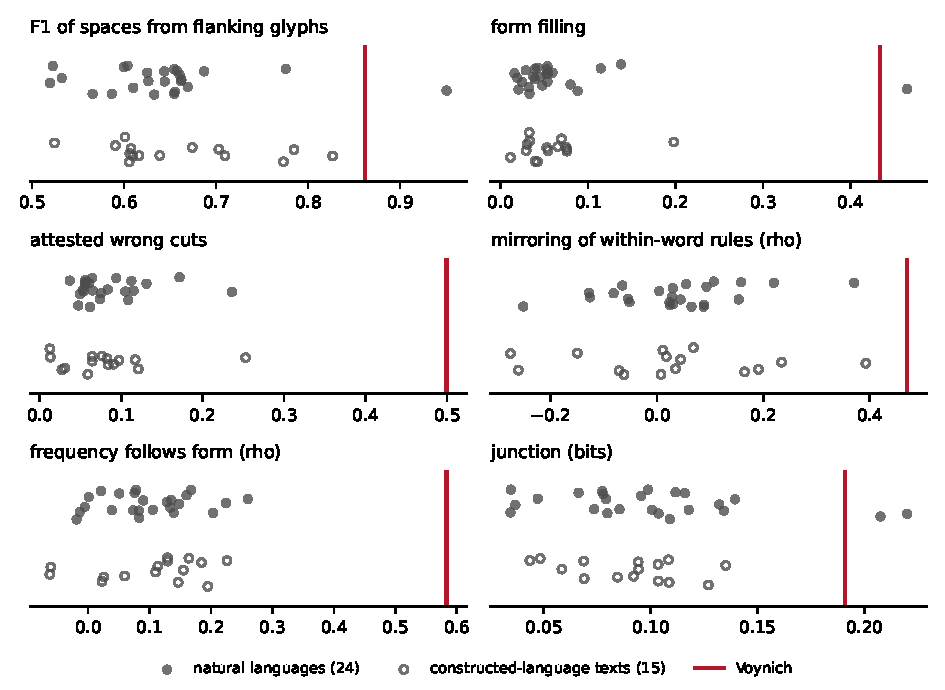
\includegraphics[width=\linewidth]{figure/lingue.pdf}
\caption{The Voynich (red line) among the 24 natural languages (dots, one per language) and the constructed languages
(open circles) for six measures. Data: \expcode{e3c84}.}
\label{fig:languages}
\end{figure}

\subsection{Seventy-nine medieval manuscripts and a cipher copyist}
\label{sec:scribes}

If the rules of Section~\ref{sec:rules} were ordinary scribal habits, real scribes copying real texts would have them.
We measured the same properties, with the same code, in 79 manuscripts transcribed at the level of letter forms with
their original lines and pages: six Nordic manuscripts from about 1200 to 1550 \citep{menota} and 73 German manuscripts
from 1350 to 1500, the area and century of the Voynich, with lines of five to eight words \citep{ref2021}. A variant
choice was measured only if it occurs at least 300 times in its minority form among words that show both forms; this
rule excludes the choices that are fixed by position in the word (for example a long \emph{s} that never appears at the
end). Table~\ref{tab:battery} gives the results and Figure~\ref{fig:battery} the intervals choice by choice.

\begin{table}[htbp]
\centering\footnotesize
\caption{The scribe battery: properties of the Voynich measured identically in 79 medieval manuscripts and in the
Copiale. ``Absent with power'' means that the upper end of the 95\% interval lies below half the Voynich value
(\expcode{e3c90}).}
\label{tab:battery}
\begin{tabularx}{\linewidth}{>{\raggedright\arraybackslash}p{2.8cm}YYYYY}
\toprule
property & Voynich & 6 Nordic manuscripts & 73 German manuscripts & Copiale copyist & reading \\
\midrule
junction rule (effect / uncertainty of the choice) & 0.058 & 2 of 11 choices at 0.013--0.015, others zero & 2 of 13 at
0.001--0.005, others zero & --- & about 4 times the strongest Nordic choice, 12 times the strongest German one \\
left margin: avoiding the start of the line above & 5 starts avoided & none in 72 tests & no manuscript with 3 or more
starts avoided; 3 of 72 with one, as expected by chance & --- & not found in the manuscripts \\
line-edge forms (gain of the most typical form) & end \eva{-m} $+0.151$; start \eva{s-} $+0.098$ & $+0.016$ to $+0.025$
(abbreviations at line end, \eva{v-} at start) & $+0.019$ (line-break hyphen); $+0.012$ & --- & same kind, 4--8 times
stronger in the Voynich \\
immediate repetition, observed/expected within the line & 1.04 & 0.02--0.07 & at most 0.79 & 0 & avoided by every scribe,
not by the Voynich \\
drift along the line (per 10 glyphs) & $-0.020$ to $-0.034$ & at most 0.0075 & at most 0.008, in no common direction &
--- & no choice drifts as much; absent with power in 20 of 29 choices \\
short state of choices, at 2--3 words & $+0.09$ & \multicolumn{2}{p{5.2cm}}{absent with power in 14 of 29 choices;
not measurable in 13; present in 2: AM 302 fol \emph{ſ/s} ($+0.08$, from copying similar words) and Holm A 10
round/straight \emph{r} ($+0.05$, also between different words; uncertain)} & \textbf{rotates} homophones: $-0.18$ between adjacent
words & weaker or absent in scribes; not established as unique \\
slow state between consecutive lines & $+0.050$ & 6 of 17 choices, 5 as large as the Voynich & --- & --- & normal in
handwriting \\
\bottomrule
\end{tabularx}
\end{table}

\begin{figure}[htbp]
\centering
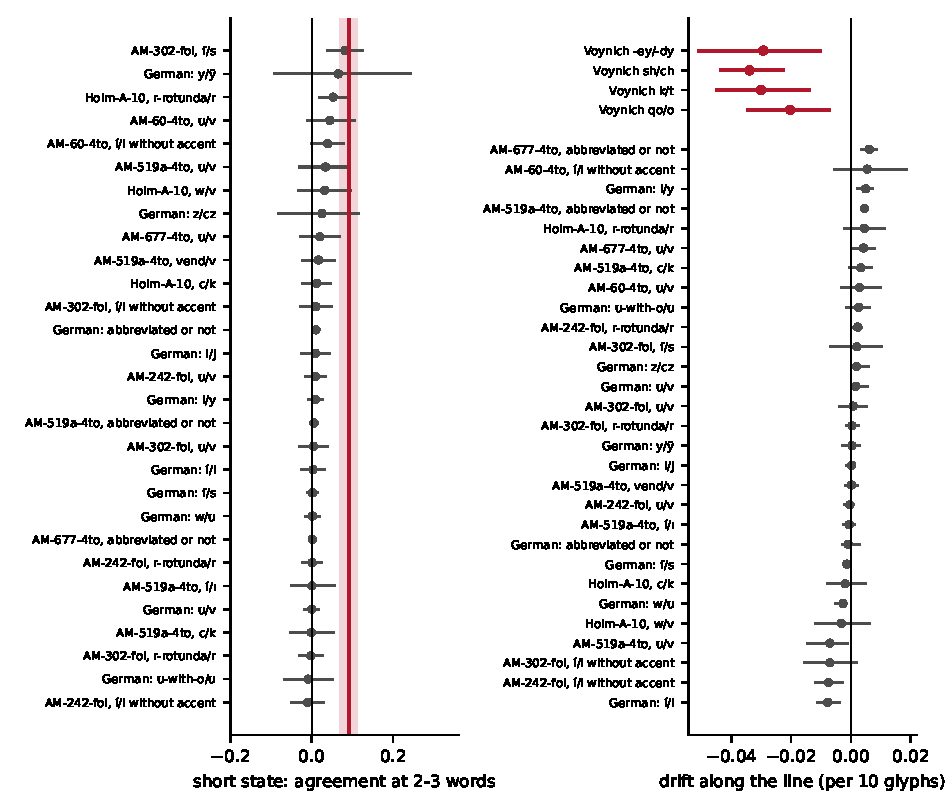
\includegraphics[width=\linewidth]{figure/scribi.pdf}
\caption{Short state (agreement at two and three words, left) and drift along the line (right) in each choice of the 79
manuscripts, with 95\% intervals, against the Voynich (red band: its 95\% interval by bifolium). Choices of the German
manuscripts are measured on the 73 manuscripts together. Data: \expcode{e3c50}, \expcode{e3c58}, \expcode{e3c62},
\expcode{e3c77}, \expcode{e3c86}, \expcode{e3c90}.}
\label{fig:battery}
\end{figure}

\paragraph{What it means} Junction rules, left-margin avoidance and the non-avoidance of immediate repetition have no
counterpart in these manuscripts; line-edge forms exist in scribes but are four to eight times weaker; the drift is
smaller in every choice (at most 0.008 against 0.020--0.034 per ten glyphs) and absent with adequate power in 20 of 29.
The short state is the property for which the comparison is weakest:
with the data available it can be called absent in only half of the choices, and the Swedish scribe of Holm A 10 shows,
in the choice between round and straight \emph{r}, an agreement half as large as the Voynich's that holds between
different words too (\expcode{e3c91}, uncertain). The slow state is normal in handwriting. The Copiale copyist does the
opposite of the Voynich: having used one symbol for a letter, he tends to use another in the next word (agreement
$-0.18$, down to $-0.48$ for \emph{u}), as one would expect from someone rotating homophones. Fifteenth-century German
herbals, recipe books and astrology texts written by hand repeat the adjacent word 7 to 30 times less than the Voynich,
so repetition does not come from genre.

These conclusions concern Old Norse and Early New High German manuscripts. Latin or Italian manuscripts of the fifteenth
century transcribed at the level of letter forms, the closest in place and kind to the Voynich, are not in the battery.

\subsection{Ciphers, readings and generators}
\label{sec:ciphers}

Every negative result in this subsection comes from a test that recovers the answer when it is there (positive control).

\paragraph{Encodings of real texts} We encoded real texts (Latin, Italian, the Bible, technical texts) and measured
whether they acquire the properties of the Voynich. A word-for-word code takes the letters and the vocabulary of the
Voynich but not its repetitions, page homogeneity or junction rules. Verbose ciphers in which each letter becomes a group
of two or three glyphs (450 variants) do not reach the predictability of the Voynich with words of its length. The
Naibbe cipher, in which each letter or pair of letters becomes a whole word chosen from homophonic tables, does: its
predictability and word length are close to the Voynich's, and \citet{kinnison2026} shows that it reproduces the
positional entropy profile. It does not reproduce repetitions, unique words, page homogeneity, the junction (almost zero)
or the line properties. Abbreviations, null letters and transpositions move away from the Voynich; encoded lists,
prayers and litanies take on its grain but not its anomalies.

\paragraph{Substitution readings} Homophonic substitution with spaces in 14 languages recovers 69--98\% of the words of
the controls and at most 36\% of Voynich ``words'', mostly the same three. A solver without spaces (simulated annealing
on a five-gram model of Latin trained on nine million letters, recovering 98--100\% of the keys of its positive
controls) never reliably beats the negative controls on the Voynich, whatever the glyph inventory, the grouping or the
reading direction. Further tests (85 languages with spaces; 16 vernaculars, historical languages and abbreviated Latin;
a mixed nomenclator; searches guided by plant names and months; other reading orders; pieces of words as symbols) gave
no reading; two formally positive outcomes proved to be artefacts. The order of glyphs inside words is language-like,
not anagram-like \citep[compare][]{hauerkondrak2016}.

\paragraph{Published readings} \citet{bax2014}: his recurring words do not behave as names (\eva{shor}, read as
``black'', occurs 96 times on 67 pages of all sections), and against 10{,}000 random keys his key does not beat chance on
the pages not used to build it ($p = 0.14$). \citet{vatne2021}: the reading relies on a transcription of its own; for
the 28 of 84 entries that match the reference transliteration, the claim that these words occur nowhere else is false (12
occur on other pages, as often as other paragraph-initial words); the other two thirds could not be tested.
\citet{cheshire2019}: the key reads more Romance words than chance, but any key of the same form adapted to the
manuscript does better, also on pages not used to adapt it (20 keys of 20). \citet{schechter2026}: the program,
re-implemented, gives the published figures, but a ``glossary'' of the most frequent words without any meaning covers as
much, the glossary ``reads'' 67--70\% of a text without a message, and the decoded word order is not Latin.
\citet{gatta2026}: the signal is equally present in a text without a message, and a mapping searched for on purpose does
better; the current version of the work itself concludes that the text does not behave like Hebrew. Applying a reading
to a text generated without content is simple, and we propose it as a minimum test for any announced decipherment.

\paragraph{Historical mechanisms} We looked for the signature that some encryption systems would leave, after checking on
texts enciphered on purpose that each test sees it. Several of these mechanisms are later than the vellum, so these are
tests of a kind of mechanism, not historical hypotheses. Homophones chosen by the copyist, as in the Copiale, would leave
a negative agreement between nearby words; the Voynich has a positive one. No frequent word or sign behaves like the
index letters of Alberti's cipher disk \citep[c.~1466;][]{alberti1466}. A message in the binary choices, as in Bacon's
biliteral cipher \citep{bacon1623}, restarting at each page or line, would be seen with overwhelming evidence ($z$ up to
70 in the controls) and is absent; a continuous message is out of reach of the test. The word tables of
\citet{trithemius1518} leave no rhythm of two to six words. An autokey restarting at each line is the only mechanism
tested that closes the line like the Voynich, but it destroys repetition, inflates the vocabulary (4{,}500--6{,}400
distinct words per 10{,}000, against 2{,}900) and leaves no margin avoidance.

\paragraph{Constructed languages, gibberish and generators} No constructed language has the junction rules, the line
properties or an agreement between adjacent word forms like the Voynich's. The volunteers' gibberish has no junction
(0.014), no line-edge forms, no copying from the line above and no margin avoidance (it repeats line starts). Among the
published generators we measured, Naibbe has neither junction nor line properties; the generator of
\citet{timmschinner2020} copies from too far above, has no junction closed within the line, no word-independent state,
no margin avoidance and no drift; U2 and U3 \citep{whitehatnetizen2026} do not combine the junction with a closed line.
We have not run \emph{voynich-fingerprint} \citep{sachak2026}, whose 44 statistics, reproduced on held-out folios, include
a cross-word junction computed without line breaks but no line-final forms, no vertical relation and no margin; our
statement is therefore limited to the generators measured.

% ---------------------------------------------------------------------------
\section{From measurements to a scorecard}
\label{sec:scorecard}

A generator needs a target that can be checked. The measurements were turned into four instruments, all computed on a
whole generated book and on the real manuscript in the same way.

\paragraph{The scorecard} Eighteen properties (Table~\ref{tab:scorecard}), each with a pass band around the Voynich
value. Seventeen come from the early experiments of the project and one (the line edges) from a later one; the bands were
chosen after seeing the results of those experiments, so they are a specification, not a test. The book is cut into
pseudo-pages of 29 lines. Measured in exactly this way, the real manuscript passes 17 of the 18: the band of the
``gradient'' (similarity at six lines relative to similarity within the line) was set from a different page division and
the manuscript itself scores 0.68 against a band of 0.70--0.97. We therefore count 17 attainable properties.

\paragraph{Eight extra properties} Added later from the research results (\expcode{e293}): rare words per page,
types per token and unique words within the page, the spread of word lengths, the register of the first lines of
paragraphs, the spelling choices that vary from line to line (at least 10 of 12 classes with excess variance), the
agreement of word endings, and the share of word pairs seen elsewhere in the text. The manuscript passes all eight.

\paragraph{The line gate} Five conditions that must hold together: a line rarely starts with the first glyph of the line
above (ratio at most 0.7; Voynich 0.53); the junction across the line break is below a tenth of the junction inside the
line; similarity at distance two is at least that at distance one (Voynich 1.05); at least three of the five spelling
choices vary from line to line ($z > 3$); and the correlation between consecutive lines is $0.207 \pm 0.07$.

\paragraph{Two judges} A judge is a classifier trained to tell real pages from generated ones, retrained from scratch on
every generated book; its cross-validated area under the ROC curve (AUC) is a classifier two-sample test
\citep{lopezpaz2017}. Each real page and the generated page with the same folio name are kept in the same fold
(10 folds, repeated with five seeds), on the 202 pages with at least 40 legible words. The first judge
(\expcode{e231}) is an L2-regularised logistic regression on 209 page features: frequencies of the 30 most frequent
glyphs and of the 150 most frequent glyph pairs inside words; word length; types per token and unique words; first and
last glyphs of lines; similarity of neighbouring words and attested joins; and vertical similarity. The second
(\expcode{e266}) adds 19 features: pairs seen elsewhere, identical neighbours, similarity at distance two, the length and
initials of first and last words of lines, gallows and word length in the first lines of paragraphs, and the divergence of
a page's glyphs from the book's and between the halves of the page. No feature tests whether a word belongs to the Voynich
vocabulary. An AUC of 0.5 means that the judge is guessing and 1 that it never errs; the project set in advance 0.6 or
less as ``hard to tell apart'' and 0.7 or more as ``distinguishable''. Controls: Currier's languages A and B are told apart
with AUC 1.000; random labels give 0.53 and 0.52; two earlier generators of the project give 0.97/0.99 and 0.87/0.94.

\paragraph{A ladder of controls} To read an AUC, we degraded the real manuscript one level at a time and judged it
(\expcode{e400}; Table~\ref{tab:ladder}). Shuffling the lines within each page costs nothing to the first judge and brings
the second to 0.60; shuffling the words within each line already gives 0.98--0.99; drawing the words from other pages of
the same section gives 1.00. The second judge's floor for any text without the real line order is thus about 0.60.

\begin{table}[htbp]
\centering\footnotesize
\caption{The scorecard: 18 properties measured on a whole book cut into pseudo-pages of 29 lines, with the pass band and
the value of the real manuscript. Property 7 is not attainable (the manuscript fails its band). Values of the generator
are in Table~\ref{tab:results}.}
\label{tab:scorecard}
\begin{tabularx}{\linewidth}{rYll}
\toprule
\# & property (measure) & passes if & Voynich \\
\midrule
1 & conditional entropy of the next glyph, $h_2$ & $\pm 0.15$ & 2.236 \\
2 & predictability of the space & $\pm 0.08$ & 0.664 \\
3 & share of words occurring once (at 34{,}000 words) & $\pm 0.08$ & 0.678 \\
4 & types per token, whole text & $\pm 0.04$ & 0.210 \\
5 & identical neighbours, relative to the line's composition & $\pm 0.2$ & 1.009 \\
6 & homogeneity: similarity of words within the line & $\pm 0.008$ & 0.0385 \\
7 & gradient: similarity at six lines / within the line & 0.70--0.97 & 0.683 (fails) \\
8 & junction: last glyph $\to$ first glyph & $\pm 0.05$ & 0.188 \\
9 & attested joins of neighbours, relative to chance & 1.5--2.5 & 1.97 \\
10 & flat curve of once-occurring words (1{,}000 vs 34{,}000 words) & $\le 0.10$ & 0.057 \\
11 & vocabulary turnover between near and far blocks & $\ge 0.05$ & 0.106 \\
12 & page profile (ratio and share) & 0.8--1.25 and 0.5--1.5$\times$ & 1.06; 0.061 \\
13 & autocorrelation of neighbouring word lengths & $\ge 0.08$ & 0.150 \\
14 & Zipf slope & $\pm 0.10$ & $-1.041$ \\
15 & word shape: glyphs at the first, second, second-last and last position & $\le 1.0$ & 0 \\
16 & vertical similarity: same position in the line above & $\ge 1.015$ & 1.028 \\
17 & formulas: two- and three-word sequences recurring at least ten pages apart & 0.5--1.5$\times$ & 6.39 \\
18 & line edges: divergence of line-initial and line-final glyphs & 0.5--2$\times$ & 23; 55 \\
\bottomrule
\end{tabularx}
\end{table}

\begin{table}[htbp]
\centering\footnotesize
\caption{The ladder of controls: the real manuscript, with its true layout, degraded one level at a time (means of four
seeds; \expcode{e400}).}
\label{tab:ladder}
\begin{tabularx}{\linewidth}{Yrrr}
\toprule
text & AUC judge 1 & AUC judge 2 & scorecard (of 18) \\
\midrule
the manuscript as it is & 0.500 & 0.500 & 17.0 \\
lines shuffled within each page & 0.481 & 0.595 & 17.0 \\
words shuffled within each line & 0.984 & 0.990 & 11.5 \\
words shuffled within the page & 0.989 & 0.998 & 11.2 \\
words drawn from the other pages of the same section and language & 0.998 & 1.000 & 6.2 \\
words drawn from the other pages of the book & 1.000 & 1.000 & 5.0 \\
the manuscript with a message forced into its five spelling choices & 0.622 & 0.630 & 16.0 \\
\bottomrule
\end{tabularx}
\end{table}

\paragraph{What the instruments leave out} Some rules of Section~\ref{sec:rules} enter the instruments only indirectly
(the drift along the line, the short state of choices, the bifolium as a unit) or not at all (closure at the gap of a
drawing, the labels). The instruments were built by the project and the generator was tuned against them; an
independently built judge has not been tried (Section~\ref{sec:limits}).

% ---------------------------------------------------------------------------
\section{The voynichizer}
\label{sec:generator}

The voynichizer \citep{voynichizer} takes any text in UTF-8 and a key, and writes a book with the 207 folio names,
sections and Currier languages of the manuscript, about 4{,}050--4{,}260 lines in EVA transliteration. With the key the
text comes back exactly; with a wrong key it is rejected. This section describes version~21, the published one.
Figure~\ref{fig:pipeline} gives the overall design and Figure~\ref{fig:page} an example.

\begin{figure}[htbp]
\centering
\begin{tikzpicture}[font=\footnotesize,
  box/.style={draw, rounded corners=2pt, align=center, inner sep=3pt, minimum height=10mm, text width=#1},
  box/.default=22mm,
  key/.style={draw, dashed, rounded corners=2pt, align=center, inner sep=3pt, minimum height=7mm, text width=14mm},
  arr/.style={-{Stealth[length=2mm]}, thick}]
\node[box=16mm] (msg) at (0,0) {text\\(any language)};
\node[box=24mm] (enc) at (2.85,0) {compress, frame, encrypt, authenticate};
\node[box=17mm] (dec) at (5.85,0) {arithmetic decoder};
\node[box=25mm] (cnt) at (8.95,0) {how many times each known word appears on each page};
\node[box=15mm] (book) at (12.05,0) {book of 207 folios, EVA};
\node[key] (k) at (2.85,2.0) {key};
\node[box=46mm] (model) at (7.4,2.0) {model of the manuscript: lexicon of each section and language, character of a
real page, invented words};
\node[box=26mm] (arr) at (8.95,-2.0) {layout and word order (no information)};
\node[box=26mm] (spec) at (3.6,-2.0) {scorecard, line gate, judges (Section~\ref{sec:scorecard})};
\draw[arr] (msg) -- (enc);
\draw[arr] (enc) -- node[above]{bits} (dec);
\draw[arr] (dec) -- (cnt);
\draw[arr] (cnt) -- (book);
\draw[arr] (k) -- (enc);
\draw[arr] (k) -- (model);
\draw[arr] (model.south -| dec.north) -- node[left]{probabilities} (dec.north);
\draw[arr] (arr) -| (book);
\draw[arr, dashed] (spec) -- node[above]{tuned against} (arr);
\end{tikzpicture}
\caption{Design of the voynichizer. The encrypted bits only decide the word counts of each page, through an arithmetic
decoder that samples them from the model; everything else comes from the key and the manuscript's statistics. Reading
runs the arithmetic encoder on the observed counts.}
\label{fig:pipeline}
\end{figure}

\subsection{Design principle}

Feeding uniformly random bits to an arithmetic decoder produces an exact sample of the decoder's probability model, up to
the quantisation of the probabilities. If the bits are the ciphertext of a message under a good cipher, they are
indistinguishable from random bits, and the book is a sample of the model whether or not it carries a message: security
relative to the model in the sense of \citet{cachin1998}, by the method of \citet{ziegler2019}. Two consequences follow.
The model, not the message, decides how close the book comes to the manuscript; and the capacity is fixed by the entropy
of the part of the model that carries the bits, and cannot be raised without changing the statistics.

\subsection{From text to bits}

The text is compressed with zlib and framed as \emph{length} (4 bytes) $\|$ \emph{tag} (8 bytes) $\|$
\emph{compressed text}, where the tag is a truncated HMAC-SHA256. The frame is XORed with a SHAKE-256 keystream; after
it, the same keystream continues as filler, so that a book without a message is driven by the keystream alone. The
master key is derived with scrypt ($n = 2^{15}$, $r = 8$, $p = 1$) from the passphrase; each random choice of the
program has its own generator seeded from an HMAC of the master key and the use (and the page, for the choices made
page by page). For example, the opening of
Book~XVII of Isidore's \emph{Etymologiae} (11{,}207 bytes) compresses to 4{,}776 bytes and becomes 38{,}304 framed bits.

\subsection{The model of the book}

\paragraph{Layout} For each page type (section and Currier language), the program keeps the number of lines per page, the
page width (median words per line) and paragraph lengths, and for the whole book the ratio of words in a line to the
page width by line role (first, middle, last, only line of a paragraph). It draws a page from these statistics, so no
generated page copies the layout of a real one; books come out about 5\% longer than the manuscript.

\paragraph{Known and invented words} About 86\% of the manuscript's running words are \emph{known} words (2{,}246 types
that occur at least twice); the rest occur once. In each of eight place classes (first line of a paragraph or not, times
first, second, middle or last word of the line) a place receives an invented word with the probability observed for
once-occurring words in that class in the manuscript, adjusted by the page. Invented words are generated by a glyph model
(each glyph predicted from the three before it, backing off to two) learned on the 4{,}776 once-occurring words, with
lengths drawn by place class; an invented word of six glyphs or more is, with probability 0.25, replaced if possible by
a join of two known words of the page whose junction is probable. An invented word is never a Voynich word,
so it cannot be confused with a known one when reading.

\paragraph{The lexicon of a page and its ``character''} The known-word lexicon of a page is made of the occurrences of
known words on the other pages of the same section and language (never the page itself). The key chooses another real
page of the same type, whose glyph frequencies give the page its ``character'': each word's weight is its count raised to
$\gamma = 0.976$, times $\exp(\kappa \sum_g n_g(w)\,\delta_g)$, where $\delta_g$ is the smoothed log-ratio of glyph $g$
between the chosen page and its section and $\kappa = 0.644$.

\subsection{The channel: word counts}

The bits decide only how many times each known word appears on each page. For a page with $n$ known-word places and
ordered integer weights $w_1 \ge \dots \ge w_m$ (total $W$), the counts are one multinomial draw, written as a chain of
binomials: $c_1 \sim \mathrm{Bin}(n, w_1/W)$, $c_2 \sim \mathrm{Bin}(n - c_1, w_2/(W - w_1))$, and so on. Each binomial
is a run of binary decisions (``stop at $j$ copies?'', with probability $P(X = j)/P(X \ge j)$ quantised to 16 bits), and
each decision is a symbol of a 32-bit binary arithmetic coder. Writing runs the coder's \emph{decoder} on the ciphertext
bits, so the decisions are sampled; reading runs its \emph{encoder} on the observed decisions and recovers the bits, then
XORs them, checks length and tag and decompresses. The bits are consumed in page order; the Isidore text fills about 130
of the 207 pages and the filler the rest.

\paragraph{Capacity} A v21 book carries 81{,}100--85{,}900 bits (mean 83{,}400 over 24 keys), about 2.7 bits per known
word, roughly 20{,}000 characters of ordinary prose after compression. The first versions hid the bits in the five
spelling choices (\eva{ch}/\eva{sh}, \eva{k}/\eva{t}, \eva{-l}/\eva{-r}, \eva{qo-}/\eva{o-}, \eva{-dy}/\eva{-ey}), with
about 0.8 bits per choice and 46{,}000 bits per book; moving the channel into the word counts nearly doubled the capacity
and made the books harder to tell apart (Table~\ref{tab:versions}).

\subsection{Arrangement: word order carries no information}

Once the multiset of words of a page is fixed, its order is chosen by a Metropolis sampler (60 proposed swaps per word,
temperature 1) on a score with thirteen terms learned or tuned on the manuscript: the affinity of each word for its place
class (a logistic model on the word's first and last glyphs, length, prefix and ending); links between neighbouring words
(ending--prefix and prefix--prefix, last glyph--first glyph, joins that form a word of the book, pairs seen on other
pages, identical neighbours); similarity with the word at the same position in the line above and with the word two
places away; avoidance of a line starting with the same glyph as the line above; agreement of the five spelling choices
within a line and between consecutive lines; a difference between the two halves of the page; and line widths. None of
these choices affects reading: moving words within a page changes nothing; adding, removing or changing a known word breaks
the reading, and there is no error correction.

\subsection{Security, as far as it goes}

The building blocks are standard, but the whole has not been reviewed by a cryptographer. The scrypt salt is fixed, so a
dictionary of guessed passphrases can be prepared once for all books; the keystream depends only on the key, so two books
written with the same key share it and a different key should be used for each message. A long random passphrase (six
random words or twelve random characters) is needed. The program hides \emph{that there is a message}, not that the
program was used: about 85\% of the running words of a book are Voynich words, and a book is recognisable as the
program's output.

\subsection{Development}

Table~\ref{tab:versions} summarises the versions that changed the method. Every version was judged on the same
instruments. From version~14 on, the numbers we cite come from keys never used for tuning; versions 17 and 20 were
released on the development keys and confirmed on the other 12 later the same day, version~21 before release.

\begin{table}[htbp]
\centering\footnotesize
\caption{Main versions of the voynichizer (AUC of the two judges; the early v8 benchmark used one key with three seeds
and is optimistic compared with later replications).}
\label{tab:versions}
\begin{tabularx}{\linewidth}{lYr}
\toprule
version & what changed & AUC judge 1 / judge 2 \\
\midrule
v0 & body from an earlier generator; message forced into the five spelling choices & 0.958 / 0.980 \\
v1 & arithmetic coding over a model of the spelling choices; about 46{,}000 bits & 0.889 / 0.957 \\
v8 & generator ``by pieces'': page lexicon, borrowed character, invented words, learned arrangement & 0.604 / 0.715 (3 seeds) \\
v10 & message moved into the word counts & 0.572 / 0.690 (12 keys) \\
v14 & joins accepted only with a probable junction & 0.575 / 0.600 (24 keys) \\
v15--v17 & authenticated encryption (scrypt, SHAKE-256, HMAC); statistical layout; first public release & 0.559 / 0.597 (24 keys) \\
v21 & correction of an initialisation defect in the arrangement (found by reading the public code) & 0.554 / 0.601 (24 keys) \\
\bottomrule
\end{tabularx}
\end{table}

\begin{figure}[p]
\centering\footnotesize
% generato da genera_figure.py: prime 12 righe di f1r (ZL) e del libro d'esempio v21
\begin{minipage}{\linewidth}
\textbf{f1r, the manuscript} (first 12 lines, ZL transliteration)\par\medskip
{\voyfont\large\raggedright\setlength{\parskip}{2pt}
fachys ykal ar ataiin shol shory cthres y kor sholdy\par
sory ckhar or y kair chtaiin shar ase cthar cthar dan\par
syaiir sheky or ykaiin shod cthoary cthes daraiin sy\par
soiin oteey oteos roloty cthiar daiin okaiin or okan\par
sair y chear cthaiin cphar cfhaiin\par
ydaraishy\par
odar cy shol cphoy oydar sh s cfhoaiin shodary\par
yshey shody okchoy otchol chocthy os chy dain chor kos\par
daiin shos cfhol shody\par
dain os teody\par
ydain cphesaiin ols cphey ytain shoshy cphodal es\par
oksho kshoy otairin oteol okan shodain sckhey daiin
\par}
\vspace{8mm}
\textbf{f1r, a book generated by version 21} (first 12 lines)\par\medskip
{\voyfont\large\raggedright\setlength{\parskip}{2pt}
ocheoporaiin shdar opchey otar cphedy opchedy aiir shkechom\par
soin ain chees oaly oiies ykdain dam chekchy daiin\par
sain olchs ar shedy oltal ched air olchdy okaiin olkeol ytor\par
ytaiin ykchedy chol tor chekain olkal ain okeedy otaiin\par
yrool ytchy oraiin airodeey lchey otain otar\par
olky al otchol okaiin chdal r qo keeo r shckhy olkey qokain or alchdy qokal okal ry\par
sain sheedy qokal shedy lkeear olkeedy qoeekeey qoky\par
ytchy kchedy dlar cheoky lol chekain chor dcheedy chaiin chedy yteol qoky soraiin dar\par
qo lchedy qokey qokaiin oteey lkeol qokaldy ain yokecheeg\par
or aiiin okaiin orkoldy\par
tody keody cheol shedy opchsd opo oteey otedo qokar oteody yfcheety\par
sain olain okain choepy shey ol okeedal cholkaly otain chey ar shedy aly
\par}
\end{minipage}

\caption{The first twelve lines of folio 1r in the manuscript (top) and in a book generated by version~21 (bottom), both
set in the voynichizer's font. The generated book hides the sentence ``This book was written by the voynichizer. Its words hide
this sentence, compressed and encrypted; without the key it reads like the Voynich manuscript and says nothing.'' It can
be read back with the public program and the key \texttt{white paper figure one, public example key}. The message uses
1{,}144 of the book's 83{,}480 bits.}
\label{fig:page}
\end{figure}

% ---------------------------------------------------------------------------
\section{Evaluation}
\label{sec:evaluation}

\paragraph{Protocol} Version~21 was run with 24 keys on the same text (the opening of Isidore's \emph{Etymologiae}
XVII, 38{,}304 bits). Keys 1--12 had also been used during development to choose between variants; keys 13--24 never
were. Each book was judged by the two judges, the scorecard, the eight extra properties and the line gate, read back with
its key and with a wrong key.

\begin{table}[htbp]
\centering\footnotesize
\caption{Version~21 on 24 keys: the instruments of Section~\ref{sec:scorecard} (mean $\pm$ standard error over keys).
Lower part: each scorecard property, Voynich value, mean of the generated books, and the number of keys whose book fails
it.}
\label{tab:results}
\begin{tabularx}{\linewidth}{Yrrr}
\toprule
 & keys 1--12 & keys 13--24 (fresh) & all 24 \\
\midrule
AUC judge 1 & $0.554 \pm 0.006$ & $0.554 \pm 0.005$ & $0.554 \pm 0.004$ (0.517--0.580) \\
AUC judge 2 & $0.596 \pm 0.008$ & $0.606 \pm 0.006$ & $0.601 \pm 0.005$ (0.551--0.632) \\
keys with judge 2 above 0.60 & 6 & 8 & 14 \\
scorecard (of 17 attainable) & 16.0 & 15.9 & 16.0 \\
extra properties (of 8) & 5.5 & 5.2 & 5.4 \\
line gate passed & 12 of 12 & 12 of 12 & 24 of 24 \\
exact read-back; wrong key rejected & 12; 12 & 12; 12 & 24; 24 \\
capacity (bits) & & & 81{,}100--85{,}900 \\
\bottomrule
\end{tabularx}

\vspace{0.6em}
\begin{tabularx}{\linewidth}{rYrrr}
\toprule
\# & scorecard property & Voynich & generated (mean) & keys failing \\
\midrule
1 & $h_2$ & 2.236 & 2.284 & 0 \\
2 & predictability of the space & 0.664 & 0.639 & 0 \\
3 & words occurring once & 0.678 & 0.738 & 0 \\
4 & types per token & 0.210 & 0.205 & 0 \\
5 & identical neighbours relative to the line & 1.009 & 0.943 & 0 \\
6 & homogeneity within the line & 0.0385 & 0.0414 & 1 \\
7 & gradient (not attainable) & 0.683 & 0.62 & 24 \\
8 & junction & 0.188 & 0.180 & 0 \\
9 & attested joins relative to chance & 1.97 & 2.13 & 0 \\
10 & flat curve of once-occurring words & 0.057 & $-0.024$ & 0 \\
11 & vocabulary turnover & 0.106 & 0.095 & 0 \\
12 & page profile (ratio) & 1.06 & 0.66 & 24 \\
13 & autocorrelation of word lengths & 0.150 & 0.142 & 0 \\
14 & Zipf slope & $-1.041$ & $-1.005$ & 0 \\
15 & word shape & 0 & 0.040 & 0 \\
16 & vertical similarity & 1.028 & 1.035 & 0 \\
17 & formulas & 6.39 & 4.58 & 0 \\
18 & line edges (start; end) & 23; 55 & 23.6; 54.5 & 0 \\
\bottomrule
\end{tabularx}
\end{table}

\begin{figure}[htbp]
\centering
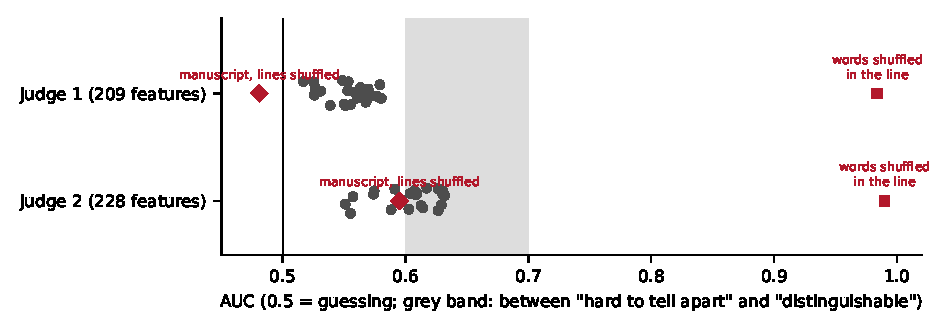
\includegraphics[width=\linewidth]{figure/valutazione.pdf}
\caption{AUC of the two judges for the books of the 24 keys (dots), against the real manuscript degraded on purpose
(red): with its lines shuffled within each page, and with its words shuffled within each line. Data:
\expcode{e409b} (version~21) and \expcode{e400}.}
\label{fig:evaluation}
\end{figure}

\paragraph{How close to the manuscript} The first judge separates generated from real pages with AUC 0.55, the second
with 0.60 (Table~\ref{tab:results}, Figure~\ref{fig:evaluation}); on the fresh keys the second judge gives 0.606. For the
second judge this is the level of the real manuscript with its lines shuffled within each page (0.595), and far from
the manuscript with its words shuffled within each line (0.99). The group of features that the second judge uses best
is the register of the first lines of paragraphs (AUC 0.62 on that group alone). The books pass 16 of the 17
attainable scorecard properties: they always miss the page profile, a measure of how much each page departs from its
section, and once the homogeneity within the line. Of the extra properties they usually miss the spelling choices that
vary from line to line (23 of 24 keys), the register of the first lines (18 of 24) and the spread of word lengths (20 of
24). Lines are too irregular in width: 11.6\% are wider than 1.25 times the page median, against 6.0\% in the
manuscript. About 0.4--0.5\% of the word triples of a book also occur in the manuscript.

\paragraph{With and without a message} [e419: with 24 keys, books with the Isidore text and books with filler only;
differences of the two judges against the manuscript, and a direct classifier between the two kinds of book.]

\paragraph{What the generator does not do} It writes only running paragraph text: no labels, no circular or radial
text, and no images (the website places the real drawings next to the generated folios). It does not model hands, and
it generates pages independently, so the bifolium effects of Section~\ref{sec:book} are absent. It models copying from
the line above by the index of the word in the line, whereas the manuscript copies by physical position. Two rules of
Section~\ref{sec:rules} that are not in the instruments, the closure at the gap of a drawing and the drift along the
line, were not targeted, and the short state only as agreement of the spelling choices within a line.

% ---------------------------------------------------------------------------
\section{Discussion}
\label{sec:discussion}

\subsection{What the generator shows}

The voynichizer is a constructive argument. Its books reproduce most of the measured writing rules of the manuscript, to
the point that two classifiers retrained on each book separate its pages from the real ones only slightly better than
chance, and every book carries an encrypted text that comes back exactly with the key. Two claims must be kept apart.
\begin{itemize}
\item \textbf{A book with a message and a book without one} are samples of the same distribution, because the message
  enters only as encrypted bits, which are indistinguishable from the random filler that drives a book without a message.
  No test on the text can separate them without the key. This holds by construction, whatever the judge, as long as the
  cipher is sound; the measurement on version~21 is in Section~\ref{sec:evaluation}.
\item \textbf{A generated book and the real manuscript} are not the same distribution. Our judges separate them a
  little (AUC 0.55 and 0.60), several properties are not reproduced, and a stronger or independently built judge would
  probably do better. How close the book comes is a measured fact about our instruments.
\end{itemize}
Together they mean that statistical regularities of the kind measured here, however strong, cannot decide by themselves
whether the Voynich manuscript carries a message: a text written under these rules can carry one, and whether it does
cannot be read from its statistics. This does not show that the manuscript carries a message. It shows that the debate
between ``meaningless'' and ``enciphered'' cannot be settled by the statistics of the text alone
\citep[compare][]{gaskellbowern2022,bowerngaskell2022,greshko2025,kinnison2026}.

\subsection{What the measurements exclude and what they leave open}

\paragraph{Excluded, with the controls described}
\begin{itemize}
\item a natural language written in an ordinary alphabet and read with a simple or homophonic substitution, in the
  languages tested;
\item the published readings we could test;
\item the historical encryption mechanisms we simulated, one at a time;
\item a text invented by hand without rules, as the volunteers' gibberish is;
\item that the rules of the manuscript are the ordinary habits of the 79 Nordic and German manuscripts we measured
  (with the reservations on the short state in Section~\ref{sec:scribes}).
\end{itemize}

\paragraph{Open} Four scenarios, which our data do not separate:
\begin{enumerate}
\item \textbf{A language written with a very artificial writing system}, in which the variant forms carry no meaning but
  follow rules of form and spaces are placed by rules of form. The junction rules are compatible with a phonetically
  written language: two of the 24 languages, Sanskrit and Tagalog, have a stronger junction.
\item \textbf{A code or cipher of an untested kind}, for example with a repertory of words or a lost key book. The
  voynichizer shows one way in which a message can hide in a text with these rules.
\item \textbf{No message}: a text produced by a procedure that can be executed by hand. Generators of this kind
  reproduce many basic properties, but none of those we measured reproduces the junction rules, the closed line and the
  margin avoidance together.
\item \textbf{A line that is a unit of content} (a verse, an entry, a recipe, a formula). It would explain at once the
  closed line, the line-edge forms and the register of first and last lines; a herbal printed one verse per line has a
  closed line too. It is compatible with any of the first three scenarios.
\end{enumerate}

\subsection{What would change our mind}

\begin{itemize}
\item A reading that passes the controls used here: one that works on the real text and not on shuffled text or on
  text generated without a message, that produces meaningful sentences on pages not used to build it, and that explains
  the junction rules, the closed line, the copying from the line above and the margin avoidance.
\item A medieval manuscript, or a historical cipher, with the same rules; in particular Latin or Italian manuscripts of
  the fifteenth century, which the battery lacks.
\item A simple procedure, executable by hand, that reproduces them all together.
\end{itemize}

\noindent A reading will need an external anchor that regularities cannot give: a text of which the manuscript is a copy,
a secure identification of many plants to use as cribs, a key found in an archive.

% ---------------------------------------------------------------------------
\section{Limitations}
\label{sec:limits}

\begin{itemize}
\item \textbf{Preregistration and exploration.} The preregistrations are internal, dated files in a public
  version-controlled history, without third-party timestamps. The programme was exploratory, and confirmations on data
  not used to form a hypothesis are few (Section~\ref{sec:methods}).
\item \textbf{Transliterations.} Everything rests on transliterations that share the line segmentation. Without checking
  the images we cannot separate what the scribe did from what the transcribers read, for example the \eva{q} that drops
  after a drawing; for uncertain spaces, the image measurements of \citet{rozanova2026} show that they are physically
  narrower.
\item \textbf{Comparison manuscripts.} Old Norse and Early New High German only; no fifteenth-century Latin or Italian
  manuscript transcribed at the level of letter forms. The files do not mark changes of hand, and the 73 German
  manuscripts were measured together for the state of the choices, so a single scribe's state could be diluted. For the
  short state the power is insufficient in 13 of 29 choices.
\item \textbf{Comparison languages.} 24 natural languages, with lines made by cutting prose; 10{,}000 words per text.
\item \textbf{Historical ciphers.} Only one real enciphered manuscript (the Copiale); the DECODE archive of early modern
  ciphers requires an account and has no reuse licence, and we found no fifteenth-century cipher there with both
  transcription and key.
\item \textbf{Gaps.} Three tests could not be run because their measures did not separate the cases on synthetic texts:
  whether the state of the choices lasts a number of words or a span of writing (glyphs), whether the states of
  different choices change at the same points, and whether the short state crosses the line break. Whether the state
  survives the gap of a drawing is undecided for lack of data.
\item \textbf{The generator.} The judges and the scorecard are the project's own, and the generator was tuned against
  them; an independently built judge has not been tried. Keys 1--12 were used during development. The books are not
  indistinguishable from the manuscript. The encryption has not been reviewed by a cryptographer, and the scrypt salt is
  fixed.
\item \textbf{Effect sizes.} Several of the properties are small in absolute terms (the short state is about 13
  percentage points of agreement between adjacent words); the look-ahead and the drift of single choices other than
  \eva{sh}/\eva{ch} do not survive the strictest multiplicity correction.
\end{itemize}

% ---------------------------------------------------------------------------
\section{Availability}

\begin{itemize}
\item \textbf{Research record} \citep{repository}: preregistrations (\texttt{preregistrazioni/}), programs
  (\texttt{esperimenti/}), results with provenance records (\texttt{risultati/}), the laboratory notebook
  (\texttt{QUADERNO.md}, in Italian), the log of all experiments (\url{white_paper/revisione/registro_esperimenti.csv})
  and the sources of this paper with the script that draws its figures. Re-running an experiment gives the same numbers.
  Copyright-protected corpora are not included and must be downloaded from their sources (Appendix~\ref{app:sources}).
\item \textbf{The voynichizer} \citep{voynichizer}: program (MIT licence), the transliteration it uses (CC0), the font, and
  a website that runs version~21 in the browser. The example book of Figure~\ref{fig:page} and its message are in the
  research repository (\url{white_paper/en/figure/}).
\end{itemize}


\bibliographystyle{plainnat}
\bibliography{references}

% ---------------------------------------------------------------------------
\appendix

\section{Definitions of the main measures}
\label{app:measures}

Notation: a line is a sequence of words $w_1,\dots,w_n$; a word is a sequence of glyphs (Section~\ref{sec:data}); $\ell(w)$
and $f(w)$ are its last and first glyph. Plug-in entropies and mutual informations are in bits. Unless stated, a null is
averaged over 50--1{,}000 permutations and $z$ is the distance of the observed value from the null mean in null standard
deviations.

\paragraph{Junction} $I = I(\ell(w_i); f(w_{i+1}))$ over all pairs of adjacent words in the same line; $E = I -
\overline{I}_{\text{null}}$, the null shuffling the words of each line (same marginals and sample size, hence the same
finite-sample bias). The variant with position (\expcode{e3c87}) shuffles $f(w_{i+1})$ among pairs with the same class of
position (index of $w_i$ in the line: 0, 1, 2, 3, 4 or more; whether $w_{i+1}$ ends the line).

\paragraph{Mirroring of within-word rules} $\mathrm{PMI}_{\text{in}}(a,b) = \log \frac{n_{\text{in}}(a,b)\,N_{\text{in}}}
{n_{\text{in}}(a\cdot)\,n_{\text{in}}(\cdot b)}$ over consecutive glyphs inside words, and $\mathrm{PMI}_{\text{x}}(a,b)$
likewise over pairs $(\ell(w_i), f(w_{i+1}))$; $\rho$ is Spearman's correlation over the cells with at least five counts in
both tables.

\paragraph{Predictability of spaces} A rule $p(\text{space}\mid a,b)$ is estimated on the first half of the lines over
all pairs of consecutive glyphs $(a,b)$ (backing off to $a$, then to the global rate); on the second half a space is
predicted when $p > 0.5$; the score is the F1 of the predicted spaces.

\paragraph{Attested wrong cuts} The glyph stream of each line is re-spaced at random with the rule above (five
re-spacings); among the pieces of at least three glyphs that do not coincide with an original word, the share that are
word types of the text (median over re-spacings).

\paragraph{Form filling and frequency--form correlation} A first-order glyph chain with start and end symbols (add-0.5
smoothing) is estimated on the word types. For each length $L = 3,\dots,7$ the $K_L$ most probable sequences are found
by exact search, $K_L$ being the number of attested types of that length; filling is the share of them that are attested.
The frequency--form correlation is Spearman's correlation, within length classes and pooled after centring the ranks,
between the per-glyph log-probability of a type and the logarithm of its frequency (types occurring at least twice).

\paragraph{Agreement of choices (short state)} For a choice $c$ with forms coded $x \in \{0,1\}$ (for example \eva{k} = 1,
\eva{t} = 0), every inner word of a line of at least six words that shows the choice is an occurrence, with its
\emph{covered word} (the word with the variant position masked), hand, page and number of glyphs $g$ written before it in
the line. Its expected value is
\[
p_a = \bar x_{\text{hand,covered}}^{(-a)} + \big(\bar x_{\text{page}}^{(-a,-b)} - \bar x_{\text{hand}}^{(-a)}\big)
      + \beta_c\,\big(g_a - \bar g_{\text{page}}^{(-a,-b)}\big),
\]
clipped to $[0.01, 0.99]$, where the superscripts mean leave-one-out (or leave-two-out) means and $\beta_c$ is the
within-stratum slope of $x$ on $g$. For pairs $(a,b)$ of occurrences of the same choice at distance $d$ words in the same
line, excluding pairs whose covered words are equal or one edit apart,
\[
K(d) = \frac{\sum_{(a,b)} \big[\mathbb{1}(x_a = x_b) - e_{ab}\big]}{\sum_{(a,b)} \big[1 - e_{ab}\big]},\qquad
e_{ab} = p_a p_b + (1-p_a)(1-p_b).
\]
Because $p$ is estimated from the same data, $K$ is biased in a way that depends on the text (by up to $+0.37$). The
corrected value is $K_{\mathrm{c}}(d) = K(d) - \overline{K}(d)$, where $\overline{K}$ is the mean of $K$ over 50 shuffles of
the values $x$ among occurrences with the same hand, choice and covered word: the shuffles keep the bias and remove any
real agreement. On synthetic texts the correction brings a text without agreement back to zero and leaves a true
agreement unchanged (\expcode{e3c48}).

\paragraph{Drift along the line} Within strata (choice $\times$ covered word), the least-squares slope of $x$ on $g$,
pooled as $\sum \mathrm{cov} / \sum \mathrm{var}$ over strata, leaving out the first and last word of each line; reported
per ten glyphs.

\paragraph{Copying from the lines above} For paragraphs of at least four lines and lines from the third on, the share of
words that have an identical word, or one at one edit, in the two lines above; the null shuffles the order of the lines
within the paragraph, so that the ``lines above'' are other lines of the same paragraph; $E = $ observed $-$ null mean.

\paragraph{Left margin} For the lines of a paragraph from the second on, with at least three words and a first word of at
least two glyphs, the number of consecutive lines whose first two glyphs coincide, divided by its mean over 1{,}000
shuffles of the order of the lines within the paragraph.

\paragraph{Repetition} The share of adjacent pairs in a line that are the same word (words of at least two glyphs) or
differ by one edit (words of at least three glyphs), and its ratio to the mean share after shuffling the words within
each line (20 shuffles), or to $\sum_w p_w^2$.

\paragraph{Intervals} Contributions are summed per page; pages are grouped by bifolium (or quire), and groups are
resampled with replacement 2{,}000 times; intervals are the 2.5th and 97.5th percentiles. For the junction the null is
recomputed inside each resample from 20 within-line shuffles stored per page, so that observed and null share the same
finite-sample bias.

\begin{table}[htbp]
\centering\footnotesize
\caption{The main tests corrected for multiplicity: Holm within seven families, and Bonferroni over the 715 experiments
logged before this test ($p < 7.0\times10^{-5}$, $|z| > 3.97$). Experiment \expcode{e3c92}.}
\label{tab:multiplicity}
\begin{tabularx}{\linewidth}{>{\raggedright\arraybackslash}p{2.8cm}Yrcc}
\toprule
family & test & statistic & Holm & Bonferroni \\
\midrule
junction & junction between adjacent words & $z = 191.7$ & yes & yes \\
 & \eva{qo-}/\eva{o-} after the previous word & $z = 19.4$ & yes & yes \\
 & \eva{-l}/\eva{-r} before the next word & $z = 12.7$ & yes & yes \\
 & look-ahead, end of the first word changes & $p = 0.0002$ & yes & no \\
 & look-ahead, next word adapts & $p < 0.0001$ & yes & no \\
line edges & \eva{-m} at line end; \eva{-r} drops & $z = 26.7$; $-13.6$ & yes & yes \\
 & \eva{y-}, \eva{s-} at line start & $z = 16.6$; $16.0$ & yes & yes \\
copying & beyond the paragraph's vocabulary & $z = 17.4$ & yes & yes \\
left margin & \eva{qo-}, \eva{o-} avoided below the same start & $z = -9.7$; $-7.0$ & yes & yes \\
 & \eva{d-}, \eva{ch-}, \eva{y-} avoided & $z = -3.8$; $-3.6$; $-3.5$ & yes & no \\
short state & adjacent; two--three words (by bifolium) & $z = 12.3$; $8.1$ & yes & yes \\
drift & \eva{sh}/\eva{ch} & $z = -6.3$ & yes & yes \\
 & \eva{qo}/\eva{o}, \eva{k}/\eva{t}, \eva{-ey}/\eva{-dy} & $z = -3.0$; $-3.9$; $-2.8$ & yes & no \\
book & bifolium identity; languages A and B & $z = 6.6$; $13.4$ & yes & yes \\
\bottomrule
\end{tabularx}
\end{table}

% ---------------------------------------------------------------------------
\section{The log of experiments}
\label{app:log}

The repository contains one row per experiment from e01 to e3c92
(\url{white_paper/revisione/registro_esperimenti.csv}), with date, question, files, outcome against the
preregistered criterion, deviation and notes, and a summary with the borderline classifications. The log was compiled
semi-automatically from the preregistrations, results and notebook; every quoted outcome was checked to appear verbatim
in the sources, and 110 borderline classifications are listed for the reader to judge.

\begin{center}\footnotesize
\begin{tabular}{lrrrrrrrr}
\toprule
series & confirmed & refuted & mixed & inconclusive & superseded & descriptive & not run & total \\
\midrule
e01--e99 & 20 & 25 & 8 & 9 & 2 & 32 & 2 & 98 \\
e100--e199 & 10 & 61 & 9 & 18 & 9 & 3 & 2 & 112 \\
e200--e299 & 18 & 66 & 4 & 5 & 9 & 6 & 7 & 115 \\
e300--e399 & 37 & 26 & 15 & 13 & 2 & 7 & 1 & 101 \\
e3a & 43 & 24 & 12 & 2 & 12 & 4 & 2 & 99 \\
e3b & 22 & 22 & 12 & 12 & 29 & 1 & 1 & 99 \\
e3c & 20 & 35 & 11 & 13 & 6 & 4 & 3 & 92 \\
\midrule
all & 170 & 259 & 71 & 72 & 69 & 57 & 18 & 716 \\
\bottomrule
\end{tabular}
\end{center}

\noindent ``Confirmed'' and ``refuted'' refer to the affirmative answer to each preregistered question. Experiments
e01--e28 were imported from earlier work and re-run, without preregistration. ``Superseded'' marks outcomes later
withdrawn or reversed (in four cases only the method was corrected and the result upheld). Of the 80 declared deviations,
19 are outcomes read differently from the literal criterion; the most consequential is \expcode{e384}, whose criterion
(set from the range of short, noisy texts) literally gave ``the junction carries over the line break as in prose'',
while the measurements show a closed line ($Q \approx 0$, against 0.49 in languages; \expcode{e3c89}).

% ---------------------------------------------------------------------------
\section{Internal checks: provisional readings corrected by later work}
\label{app:checks}

\paragraph{During the research (before version 1)}
\begin{enumerate}
\item The agreement measure was biased by up to $+0.37$ (Appendix~\ref{app:measures}). Before the correction it had
  given the Anglo-Saxon scribe of the \emph{Hatton Gospels} a ``window'' like the Voynich's, made Volapük look similar to
  the Voynich, placed the shape of the Voynich's agreement outside the range of languages (it is at the top), and suggested
  that the state travels only on occurrences of the choice.
\item The state of the choices first looked like a window of three words dropping to zero; it fades gradually (half-life
  about three words), and a slow component crosses lines.
\item A per-line ``setting'' of the choices, like a key per line, did not hold.
\item After the form-only variants of the Glen Claston transliteration we read the state as tied to words rather than to
  letter shapes; a real scribe with a window in a form-only choice made that generalisation too broad.
\item An uncorrected measure suggested that hand 1 lacks the state; corrected, all hands have it.
\item An apparent reset of the choices at the line break came from comparing with the page average (line edges have
  forms of their own).
\item The first left-margin test used a defective null; the corrected one confirms the result.
\item A share of the link between whole words attributed to the paragraph was a mechanical effect of smaller groups.
\item Rare forms seemed to be copied from the line above more than others; with the second transliteration only a trend
  remains.
\item Two formally positive reading candidates (a syllabic one and a German one) were artefacts: the first came out the
  same on the shuffled Voynich, the second changed sign with the starting points of the search.
\item Three criteria called ``absent'' an effect whose interval only touched zero; the estimates were positive and
  similar to the rest. Since then ``absent'' requires the upper end of the interval below half the reference value.
\end{enumerate}

\paragraph{Prompted by the external review of version 1}
\begin{enumerate}[resume]
\item ``71 languages'' were 71 texts, 15 of them in constructed languages; per natural language almost all comparisons
  hold, but two maxima came from Toki Pona, the junction is exceeded by two languages of 24 (not ``six of 71''), and the
  per-text junction values of version~1 came from an unsaved exploratory check with a different glyph segmentation
  (\expcode{e3c84}).
\item The ``weak space inside a chain of glyphs'' does not survive a word-grammar null: predictable spaces, attested wrong
  cuts and form filling follow from word form (\expcode{e3c85}). The junction and its mirroring of within-word rules
  survive.
\item ``Repeats the previous word more than chance'' becomes ``does not avoid repeating it, and repeated words cluster in
  the line'' (\expcode{e3c88}); ``no comparison text has this signature'' for the decline of repetition within the line was
  wrong (two languages of 20; \expcode{e3c84}).
\item The drift was said to be ``three to fifteen times'' that of the Nordic scribes; relative to the strongest scribal
  drift it is about 2.5 to 4.5 times.
\item ``Not found in any of 79 scribes'' was too strong for the short state: with adequate power it is absent in 14 of
  29 choices, and Holm A 10 shows a weaker state-like agreement (\expcode{e3c90}, \expcode{e3c91}). In the first run of
  \expcode{e3c90} the drift intervals of the Nordic scribes were read in the wrong unit (per glyph instead of per ten
  glyphs), giving 28 instead of 20 choices ``absent with power''; corrected the same day.
\item Version~1 described an early version of the voynichizer (message in the spelling choices); the published version
  carries it in the word counts.
\item Version~1 presented as new several regularities described before (Section~\ref{sec:related}).
\end{enumerate}

% ---------------------------------------------------------------------------
\section{Glossary}

\begin{description}[leftmargin=0pt,itemsep=2pt]
\item[EVA] conventional alphabet to transliterate the Voynich into Latin letters; it does not indicate sounds.
\item[glyph] a sign of the manuscript; \eva{ch}, \eva{sh} and the bench gallows count as one.
\item[gallows] the tall signs \eva{k}, \eva{t}, \eva{p}, \eva{f}.
\item[Currier languages A and B] the two varieties of writing into which the pages divide.
\item[junction] information that the last glyph of a word gives about the first glyph of the next, beyond chance.
\item[junction rule] a rule linking the form of a word to its neighbour (sandhi-like).
\item[variant forms] pairs of words that differ by one glyph in a fixed position (for example \eva{k}/\eva{t}).
\item[short state] the tendency to repeat the same variant for a few words.
\item[scorecard] the 18 properties with pass bands that the generator must reproduce.
\item[judge] a classifier retrained on each generated book to tell its pages from the real ones; its AUC is a classifier
  two-sample test.
\item[AUC] area under the ROC curve: 0.5 for guessing, 1 for perfect separation.
\item[arithmetic decoder] the inverse of an arithmetic coder; fed with random bits it samples from a probability model.
\item[preregistration] a dated description, written before running, of question, data, measure and criterion.
\item[95\% interval] a bootstrap percentile interval: the range of the middle 95\% of the estimates over resamples of
  bifolia (or pages).
\end{description}

% ---------------------------------------------------------------------------
\section{Data sources and licences}
\label{app:sources}

\begin{center}\footnotesize
\begin{tabularx}{\linewidth}{>{\raggedright\arraybackslash}p{4.5cm}Yp{3.2cm}}
\toprule
data & source & licence \\
\midrule
Voynich transliterations ZL3b, IT2a, GC2a & \citet{zandbergen_transliterations} & public domain (CC0); in the repository \\
71 meaningful texts, 38 gibberish texts & \citet{gaskellbowern2022}, released subset & modified MIT (cite the paper) \\
Bible in 100 languages & \citet{christodouloupoulos2015} & CC0 \\
Latin Library; Divinum Officium & CLTK collection; Divinum Officium project & as stated by the sources (MIT for Divinum Officium) \\
six Nordic manuscripts & \citet{menota}; each text with the editor and version in its header & CC BY-SA 4.0 \\
73 German manuscripts & \citet{ref2021}, v1.0.2 & CC BY 4.0 (Zenodo) or CC BY-SA 4.0 (file); we follow the latter \\
Copiale & \citet{knight2011,knight2012}, project page at Stockholm University & research use \\
Naibbe & \citet{greshko2025}, repository greshko/naibbe-cipher & modified MIT \\
Timm and Schinner generator & \citet{timmschinner2020} & MIT \\
U2, U3 & \citet{whitehatnetizen2026} & MIT \\
readings tested & \citet{bax2014,vatne2021,cheshire2019,schechter2026,gatta2026} & as published; Schechter: none stated, local copy not redistributed \\
\bottomrule
\end{tabularx}
\end{center}


\end{document}
